% Options for packages loaded elsewhere
\PassOptionsToPackage{unicode}{hyperref}
\PassOptionsToPackage{hyphens}{url}
\PassOptionsToPackage{dvipsnames,svgnames,x11names}{xcolor}
%
\documentclass[
  11pt,
  letterpaper,
]{scrreprt}

\usepackage{amsmath,amssymb}
\usepackage{iftex}
\ifPDFTeX
  \usepackage[T1]{fontenc}
  \usepackage[utf8]{inputenc}
  \usepackage{textcomp} % provide euro and other symbols
\else % if luatex or xetex
  \usepackage{unicode-math}
  \defaultfontfeatures{Scale=MatchLowercase}
  \defaultfontfeatures[\rmfamily]{Ligatures=TeX,Scale=1}
\fi
\usepackage{lmodern}
\ifPDFTeX\else  
    % xetex/luatex font selection
    \setmainfont[]{TeX Gyre Pagella}
\fi
% Use upquote if available, for straight quotes in verbatim environments
\IfFileExists{upquote.sty}{\usepackage{upquote}}{}
\IfFileExists{microtype.sty}{% use microtype if available
  \usepackage[]{microtype}
  \UseMicrotypeSet[protrusion]{basicmath} % disable protrusion for tt fonts
}{}
\makeatletter
\@ifundefined{KOMAClassName}{% if non-KOMA class
  \IfFileExists{parskip.sty}{%
    \usepackage{parskip}
  }{% else
    \setlength{\parindent}{0pt}
    \setlength{\parskip}{6pt plus 2pt minus 1pt}}
}{% if KOMA class
  \KOMAoptions{parskip=half}}
\makeatother
\usepackage{xcolor}
\setlength{\emergencystretch}{3em} % prevent overfull lines
\setcounter{secnumdepth}{5}
% Make \paragraph and \subparagraph free-standing
\makeatletter
\ifx\paragraph\undefined\else
  \let\oldparagraph\paragraph
  \renewcommand{\paragraph}{
    \@ifstar
      \xxxParagraphStar
      \xxxParagraphNoStar
  }
  \newcommand{\xxxParagraphStar}[1]{\oldparagraph*{#1}\mbox{}}
  \newcommand{\xxxParagraphNoStar}[1]{\oldparagraph{#1}\mbox{}}
\fi
\ifx\subparagraph\undefined\else
  \let\oldsubparagraph\subparagraph
  \renewcommand{\subparagraph}{
    \@ifstar
      \xxxSubParagraphStar
      \xxxSubParagraphNoStar
  }
  \newcommand{\xxxSubParagraphStar}[1]{\oldsubparagraph*{#1}\mbox{}}
  \newcommand{\xxxSubParagraphNoStar}[1]{\oldsubparagraph{#1}\mbox{}}
\fi
\makeatother


\providecommand{\tightlist}{%
  \setlength{\itemsep}{0pt}\setlength{\parskip}{0pt}}\usepackage{longtable,booktabs,array}
\usepackage{calc} % for calculating minipage widths
% Correct order of tables after \paragraph or \subparagraph
\usepackage{etoolbox}
\makeatletter
\patchcmd\longtable{\par}{\if@noskipsec\mbox{}\fi\par}{}{}
\makeatother
% Allow footnotes in longtable head/foot
\IfFileExists{footnotehyper.sty}{\usepackage{footnotehyper}}{\usepackage{footnote}}
\makesavenoteenv{longtable}
\usepackage{graphicx}
\makeatletter
\def\maxwidth{\ifdim\Gin@nat@width>\linewidth\linewidth\else\Gin@nat@width\fi}
\def\maxheight{\ifdim\Gin@nat@height>\textheight\textheight\else\Gin@nat@height\fi}
\makeatother
% Scale images if necessary, so that they will not overflow the page
% margins by default, and it is still possible to overwrite the defaults
% using explicit options in \includegraphics[width, height, ...]{}
\setkeys{Gin}{width=\maxwidth,height=\maxheight,keepaspectratio}
% Set default figure placement to htbp
\makeatletter
\def\fps@figure{htbp}
\makeatother
% definitions for citeproc citations
\NewDocumentCommand\citeproctext{}{}
\NewDocumentCommand\citeproc{mm}{%
  \begingroup\def\citeproctext{#2}\cite{#1}\endgroup}
\makeatletter
 % allow citations to break across lines
 \let\@cite@ofmt\@firstofone
 % avoid brackets around text for \cite:
 \def\@biblabel#1{}
 \def\@cite#1#2{{#1\if@tempswa , #2\fi}}
\makeatother
\newlength{\cslhangindent}
\setlength{\cslhangindent}{1.5em}
\newlength{\csllabelwidth}
\setlength{\csllabelwidth}{3em}
\newenvironment{CSLReferences}[2] % #1 hanging-indent, #2 entry-spacing
 {\begin{list}{}{%
  \setlength{\itemindent}{0pt}
  \setlength{\leftmargin}{0pt}
  \setlength{\parsep}{0pt}
  % turn on hanging indent if param 1 is 1
  \ifodd #1
   \setlength{\leftmargin}{\cslhangindent}
   \setlength{\itemindent}{-1\cslhangindent}
  \fi
  % set entry spacing
  \setlength{\itemsep}{#2\baselineskip}}}
 {\end{list}}
\usepackage{calc}
\newcommand{\CSLBlock}[1]{\hfill\break\parbox[t]{\linewidth}{\strut\ignorespaces#1\strut}}
\newcommand{\CSLLeftMargin}[1]{\parbox[t]{\csllabelwidth}{\strut#1\strut}}
\newcommand{\CSLRightInline}[1]{\parbox[t]{\linewidth - \csllabelwidth}{\strut#1\strut}}
\newcommand{\CSLIndent}[1]{\hspace{\cslhangindent}#1}


% Wird für die Tabelle im Titelblatt der Experten verwendet:
% Array
\usepackage{array}
% Neue Definition für Tabelleneinträge
% linksbündig mit Breitenangabe
\newcolumntype{L}[1]{>{\raggedright\arraybackslash}p{#1}} 
% zentriert mit Breitenangabe
\newcolumntype{C}[1]{>{\centering\arraybackslash}p{#1}} 
% rechtsbündig mit Breitenangabe
\newcolumntype{R}[1]{>{\raggedleft\arraybackslash}p{#1}} 

\usepackage[a4paper, margin=3cm]{geometry}

% Titles take mainfont
\addtokomafont{disposition}{\rmfamily}





\usepackage{fvextra}
\DefineVerbatimEnvironment{Highlighting}{Verbatim}{breaklines,commandchars=\\\{\}}
\makeatletter
\@ifpackageloaded{bookmark}{}{\usepackage{bookmark}}
\makeatother
\makeatletter
\@ifpackageloaded{caption}{}{\usepackage{caption}}
\AtBeginDocument{%
\ifdefined\contentsname
  \renewcommand*\contentsname{Inhaltsverzeichnis}
\else
  \newcommand\contentsname{Inhaltsverzeichnis}
\fi
\ifdefined\listfigurename
  \renewcommand*\listfigurename{Abbildungsverzeichnis}
\else
  \newcommand\listfigurename{Abbildungsverzeichnis}
\fi
\ifdefined\listtablename
  \renewcommand*\listtablename{Tabellenverzeichnis}
\else
  \newcommand\listtablename{Tabellenverzeichnis}
\fi
\ifdefined\figurename
  \renewcommand*\figurename{Abbildung}
\else
  \newcommand\figurename{Abbildung}
\fi
\ifdefined\tablename
  \renewcommand*\tablename{Tabelle}
\else
  \newcommand\tablename{Tabelle}
\fi
}
\@ifpackageloaded{float}{}{\usepackage{float}}
\floatstyle{ruled}
\@ifundefined{c@chapter}{\newfloat{codelisting}{h}{lop}}{\newfloat{codelisting}{h}{lop}[chapter]}
\floatname{codelisting}{Listing}
\newcommand*\listoflistings{\listof{codelisting}{Listingverzeichnis}}
\makeatother
\makeatletter
\makeatother
\makeatletter
\@ifpackageloaded{caption}{}{\usepackage{caption}}
\@ifpackageloaded{subcaption}{}{\usepackage{subcaption}}
\makeatother
\makeatletter
\@ifpackageloaded{tcolorbox}{}{\usepackage[skins,breakable]{tcolorbox}}
\makeatother
\makeatletter
\@ifundefined{shadecolor}{\definecolor{shadecolor}{rgb}{.97, .97, .97}}{}
\makeatother
\makeatletter
\@ifundefined{codebgcolor}{\definecolor{codebgcolor}{HTML}{F5F5F5}}{}
\makeatother
\makeatletter
\ifdefined\Shaded\renewenvironment{Shaded}{\begin{tcolorbox}[frame hidden, breakable, boxrule=0pt, colback={codebgcolor}, sharp corners, enhanced]}{\end{tcolorbox}}\fi
\makeatother

\ifLuaTeX
\usepackage[bidi=basic]{babel}
\else
\usepackage[bidi=default]{babel}
\fi
\babelprovide[main,import]{ngerman}
\ifPDFTeX
\else
\babelfont{rm}[]{TeX Gyre Pagella}
\fi
% get rid of language-specific shorthands (see #6817):
\let\LanguageShortHands\languageshorthands
\def\languageshorthands#1{}
\ifLuaTeX
  \usepackage{selnolig}  % disable illegal ligatures
\fi
\usepackage{bookmark}

\IfFileExists{xurl.sty}{\usepackage{xurl}}{} % add URL line breaks if available
\urlstyle{same} % disable monospaced font for URLs
\hypersetup{
  pdftitle={Tragverhalten von Stahlbetontragwerken},
  pdfauthor={Pascal Gitz},
  pdflang={de},
  colorlinks=true,
  linkcolor={Black},
  filecolor={Maroon},
  citecolor={Blue},
  urlcolor={Blue},
  pdfcreator={LaTeX via pandoc}}


% TITELBLATT, VERSIONSTABELLE UND SELBSTSTÄNDIGKEITSERKLÄRUNG
%--------------------------------------------------------------------------------------------------------------------


\titlehead{
\includegraphics[height=0.5cm]{../imgs/logos/logo-mse}\hfill
\includegraphics[height=0.5cm]{../imgs/logos/logo-hslu-en-col} \\ }
\subject{MASTER OF SCIENCE IN ENGINEERING\\Vertiefungsmodul II}
\title{Tragverhalten von Stahlbetontragwerken}

\subtitle
{Modellvorstellungen zur nichtlinearen Verformungsberechnung}

%\thanks{
%Version 1.0
%\hfill \today
%\hfill Hun}


\date{\large Horw, Freitag, 17. Januar 2025}
\author{Pascal Gitz}

\publishers{
	\begin{table}[H]
		\centering
		\begin{tabular}{L{2cm} L{6cm}}
			Advisor: & Prof. FH, Dr. Daniel Heinzmann \\
			Experte: & Dr. Thomas Jäger \\
		\end{tabular}
	\end{table}
}
\begin{document}
\maketitle


Hiermit erkläre ich, dass ich die vorliegende Arbeit selbstständig angefertigt und keine anderen als die angegebenen Hilfsmittel verwendet habe. Sämtliche verwendeten Textausschnitte, Zitate oder Inhalte anderer Verfasser wurden ausdrücklich als solche gekennzeichnet.\\%
%
\\%
%
Horw, 14. Juni 2024 \hfill Pascal Gitz%

\vfill
%\begin{tabular}[h]{llcr} 
    %*Version 2.0 & - Definitives Exemplar & \today & MK \\ 
    %*Version 1.0 & - Prüfungsexemplar & 22. Januar 2021 & MK \\ 
%\end{tabular}\\

% Version 2.0 - Definitives Exemplar \hfill \today \quad \quad \quad \quad \quad MK\\
Version 1.0 - Prüfungsexemplar \hfill 14. Juni 2024 \quad \quad \quad \quad \quad PG\\
Version 0.9 - Entwurf \hfill 07. Juni 2024 \quad \quad \quad \quad \quad PG\\

\newpage

\chapter*{Kurzfassung}

Diese Arbeit ist Teil einer Arbeitsserie, bestehend aus dem Vertiefungsmodul I, dem Vertiefungsmodul II und der Masterthesis. Der Kern dieser Serie ist die Beschreibung von Verformungen im Stahlbetonbau basierend auf mechanischen Modellen. In der ersten Vertiefungsarbeit wurden die Hintergründe der Modelle beleuchtet und mittels Handrechnungen an Versuchen verifiziert. In dieser Arbeit, dem Vertiefungsmodul II, werden die Ansätze aus der Vorarbeit mit kommerziellen Finite-Element-Tools (FE-Tools) kombiniert. Es werden die Softwares AxisVM-X7, RFEM-6 und IDEAStatiCa verwendet.

Eine Modellvorstellung, das Federmodell, wird aufgezeigt. Dabei werden biege- und schubstarre Stäbe in regelmässigen Abständen durch Federn gekoppelt, in denen beliebig nichtlineare Steifigkeitsbeziehungen hinterlegt werden können. Dies ermöglicht die Bestimmung nichtlinearer Verformungen. Die Steifigkeiten werden anhand der Momenten-Krümmungs-Beziehung und anhand der Steifigkeit der Schubbewehrung ermittelt. Das Modell wird an einem Einführungsbeispiel illustriert, wobei analytische Lösungen mit den FE-Ergebnissen verglichen werden. Diese zeigen, dass die Ergebnisse nahezu deckungsgleich und zufriedenstellend sind, mit minimalen numerischen Abweichungen, die auf numerische Approximationen zurückzuführen sind.

Im Anschluss wird das Modell verifiziert. In diesem Kapitel werden die Versuche aus der Vorarbeit mit dem Federmodell nachgerechnet, um identische Ergebnisse wie bei den Handrechnungen zu erzielen. An einem Dreipunktbiegeversuch werden Schub- und Biegeverformungen basierend auf nichtlinearen Stoffgesetzen ermittelt und mit den gemessenen Versuchsresultaten verglichen. Die Ergebnisse sind zufriedenstellend. An einem Vierpunktbiegeversuch werden ebenfalls Biege- und Schubverformungen bestimmt und die Anwendung des Versatzmasses aufgezeigt. Auch hier werden die Modellresultate mit den Versuchsresultaten verglichen, wobei Abweichungen erkennbar sind, die knapp akzeptabel sind. Diese Unterschiede werden auf Unschärfen in den angewendeten Stoffgesetzen zurückgeführt. Im Vergleich mit den Handrechnungen aus der Vorarbeit zeigt das Federmodell jedoch identische Ergebnisse. Die Modellverifizierung wird abschliessend als erfolgreich betrachtet.

Im Kapitel der Modellanwendung wird das Federmodell an einem vorgespannten Träger angewendet. Das Kapitel beginnt mit einer detaillierten Versuchsbeschreibung, gefolgt von der Modellbildung. Die Interpretation der Vorspannung als Einwirkung sowie der Lastfall der Pressenkräfte und das Eigengewicht werden beschrieben. Der Hauptaspekt der Analyse ist die Ermittlung der Momenten-Krümmungs-Beziehung anhand nichtlinearer Stoffgesetze. Mittels einer Querschnittsanalysesoftware werden entlang der Stabachse 136 unterschiedliche Querschnitte analysiert. Die numerischen Ergebnisse werden erfolgreich durch Handrechnungen verifiziert. Die Resultate des Modells werden mit den Versuchsmessungen verglichen, wobei ein annähernd deckungsgleicher Verlauf festgestellt wird. Lediglich im Bereich der Traglast sind Unterschiede erkennbar. Das Kapitel endet mit einem Vergleich des Federmodells mit der Compatible Stress Field Method (CSFM). Die CSFM zeigt ähnliche Resultate wie das Federmodell.

\RecustomVerbatimEnvironment{verbatim}{Verbatim}{
  showspaces = false,
  showtabs = false,
  breaksymbolleft={},
  breaklines
  % Note: setting commandchars=\\\{\} here will cause an error 
}

\renewcommand*\contentsname{Inhaltsverzeichnis}
{
\hypersetup{linkcolor=}
\setcounter{tocdepth}{1}
\tableofcontents
}
\listoffigures

\bookmarksetup{startatroot}

\chapter{Einleitung}\label{einleitung}

Bereits 1935 wurden in der damaligen SIA 112 Anforderungen an die
Durchbiegung von Stahlbetonbauteilen gestellt. Seither wurde die
Gebrauchstauglichkeit, insbesondere die Verformungen von Tragwerken, zu
einer zentralen Bemessungsgrösse. Trotz dieser elementaren Rolle im
Bemessungsablauf werden Verformungen im Stahlbetonbau in der heutigen
Baupraxis häufig nur mit groben Abschätzungen bewertet. Solche Ansätze
können zu ungenauen Prognosen führen, die sowohl die Sicherheit als auch
die Wirtschaftlichkeit von Bauprojekten beeinträchtigen. Detaillierte
Verformungsberechnungen sind in vielen modernen Statiksoftwares
implementiert und frei anwendbar. Die theoretischen Hintergründe sind
jedoch selten geläufig, und die Tools werden meist als
\emph{``Blackbox''} behandelt.

Das Ziel dieser Arbeitsserie, bestehend aus dem Vertiefungsmodul I
{[}\citeproc{ref-gitz_ansatze_2024}{1}{]}, Vertiefungsmodul II und der
Masterthesis, ist es daher, dem Leser mechanische Modelle zur Bestimmung
von Verformungen umfassend aufzuzeigen. In der Vorarbeit
{[}\citeproc{ref-gitz_ansatze_2024}{1}{]} wurden die mechanischen
Modelle detailliert beschrieben und anhand von experimentellen Versuchen
verifiziert, wobei mehrheitlich auf den Einsatz kommerzieller
Finite-Elemente-Tools (FE-Tools) verzichtet wurde. Der Fokus dieser
Arbeit liegt nun auf der Integration von FE-Tools mit den theoretischen
Grundlagen, um praktisch anwendbare Lösungen zu entwickeln. Verwendet
wird hierbei die 3D Statiksoftware AxisVM-X7 und RFEM-6, sowie die 2D
Detailstatiksoftware IDEAStatiCa. Sämtliche Analysen beziehen sich auf
Stabtragwerke.

Diese Arbeit lässt sich in drei Kernthemen unterteilen. Zuerst wird die
Modellvorstellung zur numerischen Integration kinematischer Grössen
(primär Krümmung und Schiebung) beschrieben und anhand eines
Einführungsbeispiels veranschaulicht, um die theoretischen Grundlagen
klar darzustellen. Anschliessend wird die Modellvorstellung an den
bereits gut verstandenen Versuchen aus dem Vertiefungsmodul I
verifiziert, um die Zuverlässigkeit und Genauigkeit des Modells zu
bestätigen. Abschliessend wird die Anwendung an einem vorgespannten
Träger demonstriert, um die praktische Relevanz und Anwendbarkeit des
entwickelten Modells zu zeigen. Die Arbeit wird mit einem Fazit
abgeschlossen, das eine differenzierte Betrachtung zwischen Rückblick
und Ausblick bietet und damit sowohl die erreichten Ergebnisse
zusammenfasst als auch Erweiterungen aufzeigt.

Durch diese strukturierte Herangehensweise soll ein tieferes Verständnis
für das komplexe Tragverhalten von Stahlbetontragwerken geschaffen
werden. Zudem soll eine zuverlässige Grundlage zur praktischen Anwendung
im konstruktiven Ingenieurbau gelegt werden.

\bookmarksetup{startatroot}

\chapter{Modellierungseinleitung}\label{modellierungseinleitung}

Federmodell

\section{Modellbeschreibung}\label{modellbeschreibung}

\section{Zweifeldträger}\label{zweifeldtruxe4ger}

Das Vorlesungsbeispiel verfolgt das Ziel, die Verformungen eines
Zweifeldträgers für zwei Betonstähle mit unterschiedlichen
Duktilitätsklassen aufzuzeigen.
{[}\citeproc{ref-jager_stahlbeton_2009}{2}{]}.

\begin{figure}[H]

\centering{

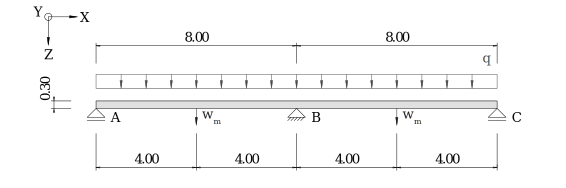
\includegraphics{A1_Traegerrost_Marti_files/mediabag/../imgs/jag_system.pdf}

}

\caption{\label{fig-jag_system}Statisches System des Zweifeldträgers mit
Abmessungen versehen}

\end{figure}%

\begin{figure}[H]

\centering{

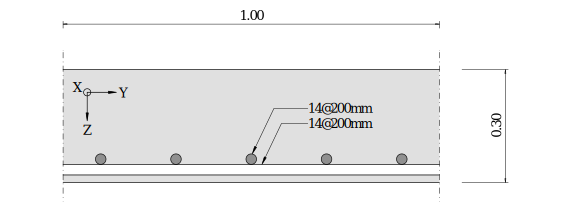
\includegraphics{A1_Traegerrost_Marti_files/mediabag/../imgs/jag_system_qs.pdf}

}

\caption{\label{fig-jag_system_qs}Querschnitt des Plattenstreifens}

\end{figure}%

\begin{figure}[H]

\centering{

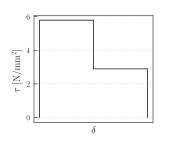
\includegraphics{A1_Traegerrost_Marti_files/mediabag/../imgs/jag_tau_delta.pdf}

}

\caption{\label{fig-jag_tau_delta}Schubspannungs-Schlupf-Beziehung als
Basis für das Zuggurtmodell}

\end{figure}%

\begin{figure}[H]

\centering{

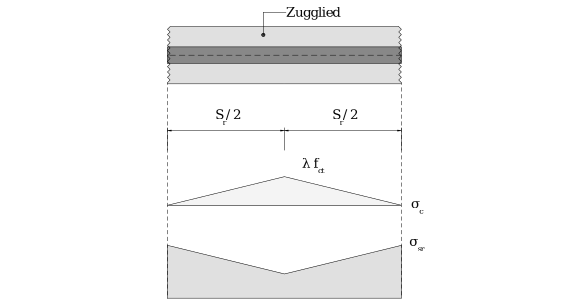
\includegraphics{A1_Traegerrost_Marti_files/mediabag/../imgs/jag_risselement.pdf}

}

\caption{\label{fig-jag_risselement}Risselement}

\end{figure}%

\begin{figure}[H]

{\centering 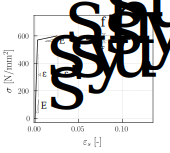
\includegraphics{A1_Traegerrost_Marti_files/mediabag/../imgs/jag_stress_strain_b500a_bearb.pdf}

}

\caption{Spannungs-Dehnungs-Beziehung des Betonstahls B500A}

\end{figure}%

\bookmarksetup{startatroot}

\chapter*{Literatur}\label{literatur}
\addcontentsline{toc}{chapter}{Literatur}

\markboth{Literatur}{Literatur}

\phantomsection\label{refs}
\begin{CSLReferences}{0}{1}
\bibitem[\citeproctext]{ref-gitz_ansatze_2024}
\CSLLeftMargin{1. }%
\CSLRightInline{Gitz P (2024) Ansätze zur {Verformungsberechnung}. HSLU
Technik \& Architektur}

\bibitem[\citeproctext]{ref-jager_stahlbeton_2009}
\CSLLeftMargin{2. }%
\CSLRightInline{Jäger T (2009) Stahlbeton {III}. Eidgenössische
Technische Hochschule Zürich}

\bibitem[\citeproctext]{ref-marti_baustatik_2014}
\CSLLeftMargin{3. }%
\CSLRightInline{Marti P (2014) Baustatik: {Grundlagen} - {Stabtragwerke}
- {Flächentragwerke}, 2., korrigierte Aufl. Ernst, Berlin}

\bibitem[\citeproctext]{ref-marti_tragverhalten_1999}
\CSLLeftMargin{4. }%
\CSLRightInline{Marti P, Alvarez M, Kaufmann W, Sigrist V (1999)
\href{https://doi.org/10.3929/ethz-a-004470343}{Tragverhalten von
{Stahlbeton}. {Fortbildungskurs} für {Bauingenieure}, {ETH} {Zürich},
30.9./1.10.1999}}

\bibitem[\citeproctext]{ref-kaufmann_2_2017}
\CSLLeftMargin{5. }%
\CSLRightInline{Kaufmann W (2017) 2 {Scheiben} und {Träger}.
Eidgenössische Technische Hochschule Zürich}

\bibitem[\citeproctext]{ref-alvarez_einfluss_1998}
\CSLLeftMargin{6. }%
\CSLRightInline{Alvarez M (1998)
\href{https://doi.org/10.3929/ethz-a-002000033}{Einfluss des
{Verbundverhaltens} auf das {Verformungsvermögen} von {Stahlbeton}}.
Birkhäuser, Basel}

\bibitem[\citeproctext]{ref-thoma_plattenversuche_2010}
\CSLLeftMargin{7. }%
\CSLRightInline{Thoma K, Niederberger I (2010) Plattenversuche an
netzbewehrten {Platten}. Hochschule Luzern Technik \& Architektur,
Technikumstrasse 21 6048 Horw}

\end{CSLReferences}

\cleardoublepage
\phantomsection
\addcontentsline{toc}{part}{Anhang}
\appendix

\chapter{Torsionsweicher
Träggerrost}\label{torsionsweicher-truxe4ggerrost}

Das folgende Beispiel ist aus
{[}\citeproc{ref-marti_baustatik_2014}{3}{]} entnommen. Dieses dient als
einführendes Beispiel in die Modellierung von Trägerrosten mit dem
Federmodell. In der Abbildung~\ref{fig-trm_uebersicht} ist der Grundriss
des Trägerrosts dargestellt. Es handelt sich um insgesamt 16
torsionsweiche Stäbe, welche an den Enden eingespannt sind.

\begin{figure}[H]

\centering{

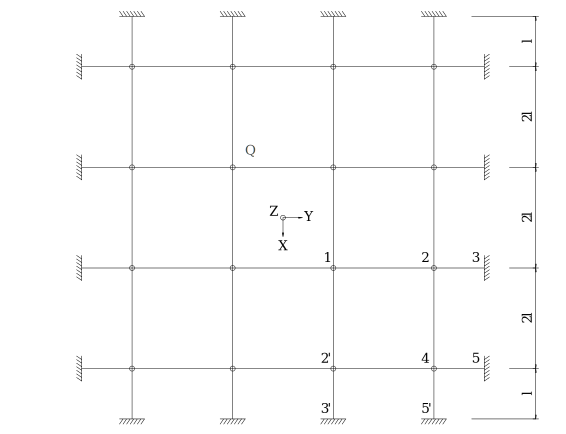
\includegraphics{A1_Traegerrost_Marti_files/mediabag/../imgs/trm_uebersicht.pdf}

}

\caption{\label{fig-trm_uebersicht}Grundriss des torsionsweichen
Trägerrosts, neugezeichnet nach
{[}\citeproc{ref-marti_baustatik_2014}{3}{]}}

\end{figure}%

Im Beispiel wird eine analytische Lösung zur Traglast aufgezeigt. Das
Ziel ist es, mittels dem Federmodell eine numerische Lösung des unteren
Grenzwerts der Traglast zu erhalten.

\section{Analytische Lösung}\label{analytische-luxf6sung}

Die Analytische Lösung basiert auf dem Traglastverfahren. Mittels einem
zulässigen Mechanismus wird ein oberer Grenzwert der Traglast
hergeleitet. In der Abbildung~\ref{fig-trm_schnitt} sind zwei Stäbe
dargestellt. Aus symmetriegründen lässt sich der obere Grenzwert des
gesamten Trägerrosts anhand dieser Darstellung ermitteln.

\begin{figure}[H]

\centering{

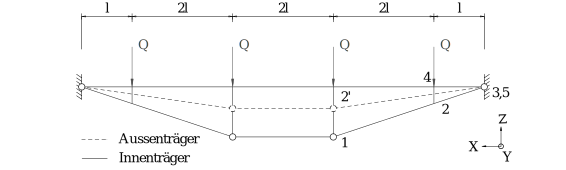
\includegraphics{A1_Traegerrost_Marti_files/mediabag/../imgs/trm_schnitt.pdf}

}

\caption{\label{fig-trm_schnitt}Schnitt des torsionsweichen Trägerrosts,
mit dem angenommenen Mechanismus für den Innen- und Aussenträger}

\end{figure}%

Die äussere Arbeit \(W_a\) des dargestellten Systems in
Abbildung~\ref{fig-trm_schnitt} beträgt dabei für die am Rand gelegenen
Stäbe (Punkte 2'45):

\[
W_{a,2'45} = 4 \cdot \left( Q \cdot \frac{1}{3} + Q \cdot \frac{1}{9} \right)
\]

Und für die Innenträger:

\[
W_{a,123} = 4 \cdot \left( Q \cdot 1 + Q \cdot \frac{1}{3} \right)
\]

Sowie beträgt die innere Arbeit:

\[
W_i = 8 \cdot \left(M_u' + M_u\right) \cdot \left(\frac{1}{3l} +\frac{1}{9l}\right)
\]

Durch das abschliessende Gleichsetzen der Arbeiten und das Lösen nach
\(Q\) folgt der obere Grenzwert der Traglast zu:

\[
Q = \frac{M_u + M_u'}{2 \cdot l}
\]

Die Plastizitätskontrolle ist in der Abbildung~\ref{fig-trm_schnitt_my}
und Abbildung~\ref{fig-trm_schnitt_vz} gezeigt. Dabei wird eine
Lastverteilung von je einer Hälfte \(Q\) in \(x\) und \(y\) Richtung
angenommen. Welche sich nach vollständigen Umlagern der Biegemomente
einstellt.

\begin{figure}[H]

\centering{

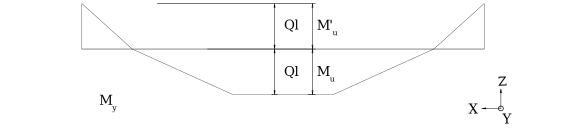
\includegraphics{A1_Traegerrost_Marti_files/mediabag/../imgs/trm_schnitt_my.pdf}

}

\caption{\label{fig-trm_schnitt_my}Plastizitätskontrolle anhand der
Schnittgrössen der Biegemomente}

\end{figure}%

\begin{figure}[H]

\centering{

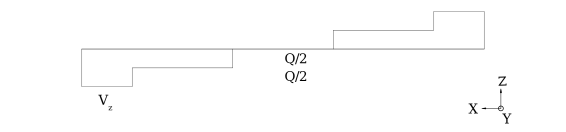
\includegraphics{A1_Traegerrost_Marti_files/mediabag/../imgs/trm_schnitt_vz.pdf}

}

\caption{\label{fig-trm_schnitt_vz}Plastizitätskontrolle anhand der
Schnittgrössen der Querkräfte}

\end{figure}%

Aus der Plastizitätskontrolle geht heraus, dass der Biegewiderstand
nirgends überschritten wird, somit deckt sich der untere und obere
Grenzwert der Traglast, sprich die Traglast \(Q_u\) wurde gefunden.

\[
Q_u = \frac{M_u + M_u'}{2 \cdot l}
\]

\section{Numerische Lösung}\label{numerische-luxf6sung}

Abschliessend wird die analytische Lösung mit der numerischen Lösung
verglichen. Dabei wird ein Federmodell erstellt. Zunächst sind die
Variablen mit numerischen Werten zu substituieren:

\[
\begin{aligned}
l& = 1 \ \mathrm{m} \quad & M_{u}& = 100 \ \mathrm{kN} \cdot \mathrm{m} \quad & {M}'_{u}& = 100 \ \mathrm{kN} \cdot \mathrm{m} \end{aligned}
\]

\[
\begin{aligned}
Q_{u}& = \frac{M_{u} + {M}'_{u}}{2 \cdot l} = 100.0 \ \mathrm{kN} \end{aligned}
\]

Der Trägerrost wurde mittels dem Federmodell nachmodelliert. Dabei sind
biegestarre, jedoch torsionsweiche Stäbe mittels Stabendgelenken
gekoppelt. Dargestellt in der Abbildung~\ref{fig-trm_geom}.

\begin{figure}[H]

\centering{

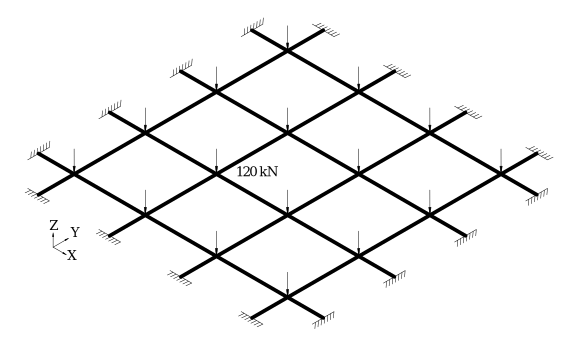
\includegraphics{A1_Traegerrost_Marti_files/mediabag/../imgs/trm_system.pdf}

}

\caption{\label{fig-trm_geom}Statisches Modell in AxisVM des
Trägerrosts}

\end{figure}%

\begin{figure}[H]

\centering{

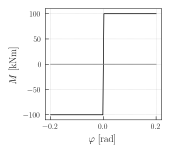
\includegraphics{A1_Traegerrost_Marti_files/mediabag/../imgs/trm_gelenkdef.pdf}

}

\caption{\label{fig-trm_gelenkdef}Ideal-plastisches
Momenten-Verdrehungs-Verhalten der Gelenke}

\end{figure}%

Den Gelenken wurde die Defintion gemäss
Abbildung~\ref{fig-trm_gelenkdef} hinterlegt. Dabei wurde der
Biegewiderstand in positiver und negativer Dimension angesetzt, ab dem
Erreichen des Biegewiderstands fliesst das Gelenk. Dies führt dazu, dass
sich die Biegemomente umlagern, sprich der Biegewiderstand auch in
Trägermitte erreicht werden kann.

\begin{figure}[H]

\centering{

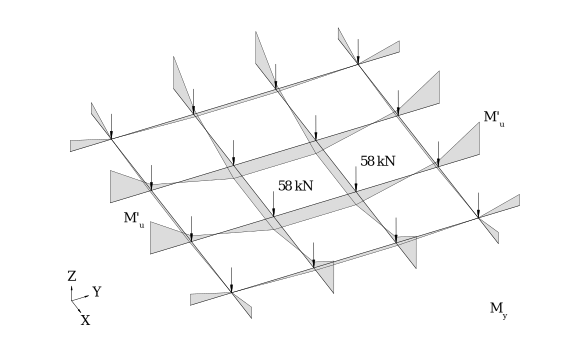
\includegraphics{A1_Traegerrost_Marti_files/mediabag/../imgs/trm_my58.pdf}

}

\caption{\label{fig-trm_my58}Biegemomente des Trägerrosts bei einer
Belastung von 58 un.kN, erste plastische Gelenke entstehen bei der
Lagerung der Innenträger}

\end{figure}%

\begin{figure}[H]

\centering{

\includegraphics{A1_Traegerrost_Marti_files/mediabag/../imgs/trm_my88.pdf}

}

\caption{\label{fig-trm_my88}Biegemomente des Trägerrosts bei einer
Belastung von 88 un.kN, plastische Gelenke entstehen bei der Lagerung
der Aussenträger}

\end{figure}%

\begin{figure}[H]

\centering{

\includegraphics{A1_Traegerrost_Marti_files/mediabag/../imgs/trm_my94.pdf}

}

\caption{\label{fig-trm_my94}Biegemomente des Trägerrosts bei einer
Belastung von 94 un.kN, plastische Gelenke entstehen im Feld der
Innenträger}

\end{figure}%

\begin{figure}[H]

\centering{

\includegraphics{A1_Traegerrost_Marti_files/mediabag/../imgs/trm_my100.pdf}

}

\caption{\label{fig-trm_my100}Biegemomente des Trägerrosts bei einer
Belastung von 100 un.kN, plastische Gelenke entstehen im Feld der
Aussenträger}

\end{figure}%

\begin{figure}[H]

\centering{

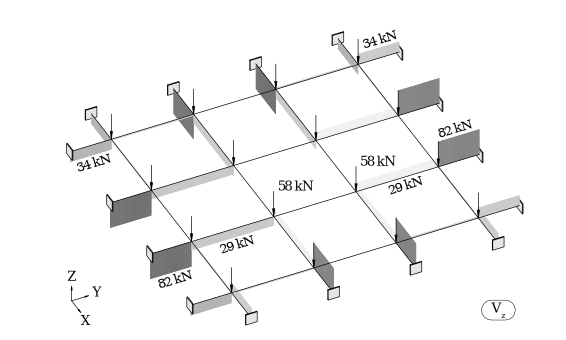
\includegraphics{A1_Traegerrost_Marti_files/mediabag/../imgs/trm_vz58.pdf}

}

\caption{\label{fig-trm_vz58}Querkräfte des Trägerrosts bei einer
Belastung von 58 un.kN, erste plastische Gelenke entstehen bei der
Lagerung der Innenträger}

\end{figure}%

\begin{figure}[H]

\centering{

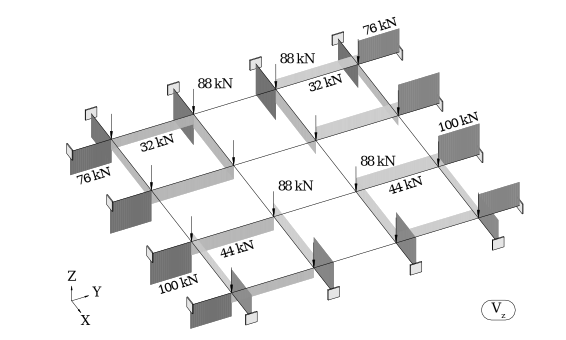
\includegraphics{A1_Traegerrost_Marti_files/mediabag/../imgs/trm_vz88.pdf}

}

\caption{\label{fig-trm_vz88}Querkräfte des Trägerrosts bei einer
Belastung von 88 un.kN, plastische Gelenke entstehen bei der Lagerung
der Aussenträger}

\end{figure}%

\begin{figure}[H]

\centering{

\includegraphics{A1_Traegerrost_Marti_files/mediabag/../imgs/trm_vz94.pdf}

}

\caption{\label{fig-trm_vz94}Querkräfte des Trägerrosts bei einer
Belastung von 94 un.kN, plastische Gelenke entstehen im Feld der
Innenträger}

\end{figure}%

\begin{figure}[H]

\centering{

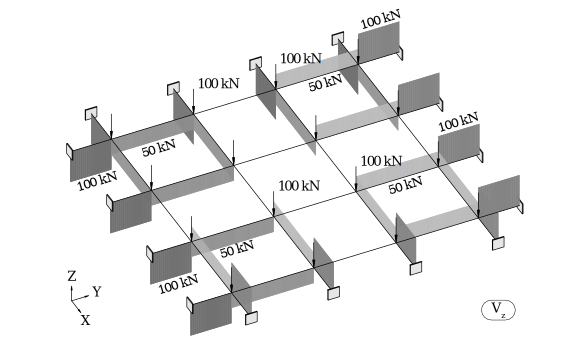
\includegraphics{A1_Traegerrost_Marti_files/mediabag/../imgs/trm_vz100.pdf}

}

\caption{\label{fig-trm_vz100}Querkräfte des Trägerrosts bei einer
Belastung von 100 un.kN, plastische Gelenke entstehen im Feld der
Aussenträger}

\end{figure}%

Mit der Belastung aus dem unteren Grenzwert stellen sich exakt die
Extremwerte der Biegemomente \(M_u\) und \(M'_u\) in den innen liegenden
Stäben ein. Das Federmodell liefert den exakten unteren Grenzwert der
Traglast. Dargestell in der Abbildung~\ref{fig-trm_my100}.

\chapter{Einführungsbeispiel -
Zweifeldträger}\label{einfuxfchrungsbeispiel---zweifeldtruxe4ger}

Um den Lesefluss aufrecht zu erhalten, werden im Anhang Bilder
wiederholt, anstelle auf den Text zu verweisen.

Das Vorlesungsbeispiel verfolgt das Ziel, die Verformungen eines
Zweifeldträgers für zwei Betonstähle mit unterschiedlichen
Duktilitätsklassen aufzuzeigen.
{[}\citeproc{ref-jager_stahlbeton_2009}{2}{]}.

\begin{figure}[H]

\centering{

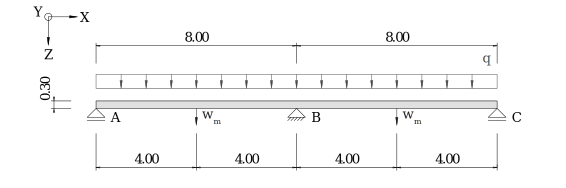
\includegraphics{A1_Traegerrost_Marti_files/mediabag/../imgs/jag_system.pdf}

}

\caption{\label{fig-jag_system}Statisches System des Zweifeldträgers mit
Abmessungen versehen}

\end{figure}%

\begin{figure}[H]

\centering{

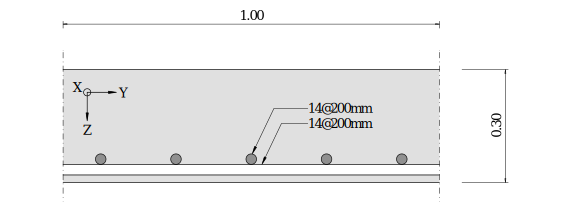
\includegraphics{A1_Traegerrost_Marti_files/mediabag/../imgs/jag_system_qs.pdf}

}

\caption{\label{fig-jag_system_qs}Querschnitt des Plattenstreifens}

\end{figure}%

Zunächst wird die analytische Lösung vollumfänglich dargestellt und mit
numerischen Werten substituiert. Abschliessend wird das
Verformungsverhalten mit dem Federmodell nachmodelliert, bzw. numerisch
approximiert.

\section{Allgemeines}\label{allgemeines}

\subsection{Annahmen}\label{annahmen}

\begin{itemize}
\tightlist
\item
  Zwei unterschiedliche Stähle
\item
  konstant gerissene Biegesteifigkeit entlang der Stabachse
\end{itemize}

\subsection{Parameter}\label{parameter}

\subsubsection{Bewehrung}\label{bewehrung}

Zunächst folgen die Parameter der Bewehrung mit den entsprechenden
Symbolbezeichnungen

\[
\begin{aligned}
\oslash_{x}& = 14 \ \mathrm{mm} \quad & s_{x}& = 200 \ \mathrm{mm} \quad & \oslash_{y}& = 12 \ \mathrm{mm} \\ 
s_{y}& = 200 \ \mathrm{mm} \quad &  \quad &  
 \end{aligned}
\]

Der Querschnitt der Längsbewehrung für den Meterstreifen beträgt dabei:

\[
\begin{aligned}
a_{s}& = \frac{\pi \cdot \oslash_{x}^{2}}{4 \cdot s_{x}} = 769.69 \ \frac{\mathrm{mm}^{2}}{\mathrm{m}} \quad &  \quad &  
 \end{aligned}
\]

\subsubsection{Geometrie}\label{geometrie}

Die verwendeten Parameter der Geoemtrie sind hier gezeigt.

\[
\begin{aligned}
c& = 20 \ \mathrm{mm} \quad & h& = 300 \ \mathrm{mm} \quad & b_{w}& = 1 \ \mathrm{m} \\ 
l& = 8 \ \mathrm{m} \quad &  \quad &  
 \end{aligned}
\]

Daraus lässt sich die statische Höhe der Längsbeweherung in
\(X\)-Richtung bestimmen:

\[
\begin{aligned}
d_{x}& = - \frac{1 \cdot \oslash_{x}}{2} - \oslash_{y} - c + h = 261.0 \ \mathrm{mm} \quad &  \quad &  
 \end{aligned}
\]

\subsubsection{Beton}\label{beton}

Für den Beton gilt die Zylinderdruckfestigkeit, der Elastizitätsmodul
und die Bruchstauchung:

\[
\begin{aligned}
f_{cc}& = 30.0 \ \frac{\mathrm{N}}{\mathrm{mm}^{2}} \quad & E_{c}& = 29.3 \ \frac{\mathrm{kN}}{\mathrm{mm}^{2}} \quad & \varepsilon_{cu}& = 5 \ \mathrm{‰} \end{aligned}
\]

Daraus wird mit empirischen Ansätzen eine Bauteilfestigkeit und eine
Betonzugfestigkeit bestimmt.

\[
\begin{aligned}
f_{ct}& = 0.3 \cdot f_{cc}^{\frac{2}{3}} = 2.9 \ \frac{\mathrm{N}}{\mathrm{mm}^{2}} \\ 
f_{c}& = 2.5 \cdot f_{cc}^{\frac{2}{3}} = 24.14 \ \frac{\mathrm{N}}{\mathrm{mm}^{2}} \end{aligned}
\]

\subsection{Modellbildung -
Zuggurtmodell}\label{modellbildung---zuggurtmodell}

Schubspannungs-Schlupf-Beziehung

\[
\begin{aligned}
\tau_{b0}& = 2 \cdot f_{ct} = 5.79 \ \frac{\mathrm{N}}{\mathrm{mm}^{2}} \\ 
\tau_{b1}& = f_{ct} = 2.9 \ \frac{\mathrm{N}}{\mathrm{mm}^{2}} \end{aligned}
\]

\begin{figure}[H]

\centering{

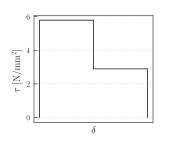
\includegraphics{A1_Traegerrost_Marti_files/mediabag/../imgs/jag_tau_delta.pdf}

}

\caption{\label{fig-jag_tau_delta}Schubspannungs-Schlupf-Beziehung als
Basis für das Zuggurtmodell}

\end{figure}%

\[
\begin{aligned}
h_{eff}& = 2 \cdot \left(- d_{x} + h\right) = 78.0 \ \mathrm{mm} \\ 
\rho& = \frac{a_{s}}{h_{eff}} = 0.99 \ \mathrm{\%} \end{aligned}
\]

\begin{figure}[H]

\centering{

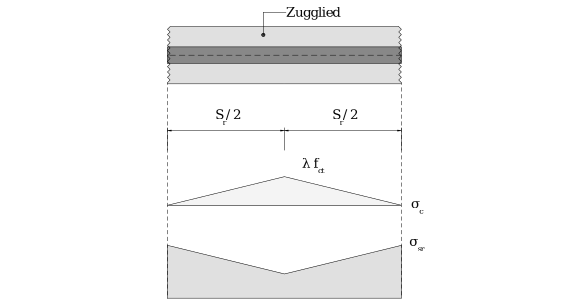
\includegraphics{A1_Traegerrost_Marti_files/mediabag/../imgs/jag_risselement.pdf}

}

\caption{\label{fig-jag_risselement}Risselement}

\end{figure}%

\[
\begin{aligned}
s_{r0}& = \frac{\oslash_{x} \cdot \left(1 - \rho\right)}{4 \cdot \rho} = 351.19 \ \mathrm{mm} \\ 
s_{rl}& = 1 \cdot \frac{1}{2} \cdot s_{r0} = 175.59 \ \mathrm{mm} \end{aligned}
\]

\[
\begin{aligned}
s_{r}& = 200 \ \mathrm{mm} \quad &  \quad &  
 \end{aligned}
\]

\section{Kaltverformter Betonstahl -
B500A}\label{kaltverformter-betonstahl---b500a}

\subsection{Eigenschaften des
Betonstahls}\label{eigenschaften-des-betonstahls}

Allgemein werden die Eigenschaften für den Betonstahl B500A mit einem
Suffix \(A\) gekennzeichnet.

\[
\begin{aligned}
f_{sy , A}& = 570.0 \ \frac{\mathrm{N}}{\mathrm{mm}^{2}} \quad & f_{su , A}& = 600.0 \ \frac{\mathrm{N}}{\mathrm{mm}^{2}} \quad & \varepsilon_{sy , A}& = 2.78 \ \mathrm{‰} \\ 
\varepsilon_{su , A}& = 25 \ \mathrm{‰} \quad & E_{s , A}& = 205.0 \ \frac{\mathrm{kN}}{\mathrm{mm}^{2}} \quad & E_{sh , A}& = 1350.0 \ \frac{\mathrm{N}}{\mathrm{mm}^{2}} \end{aligned}
\]

\begin{figure}[H]

{\centering 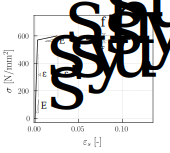
\includegraphics{A1_Traegerrost_Marti_files/mediabag/../imgs/jag_stress_strain_b500a_bearb.pdf}

}

\caption{Spannungs-Dehnungs-Beziehung des Betonstahls B500A}

\end{figure}%

\subsection{Linear elastische - gerissene
Biegesteifigkeit}\label{linear-elastische---gerissene-biegesteifigkeit}

Wird fortan für sämtliche Verformungsberechnungen verwendet.
Querschnittsanalyse:

\begin{figure}[H]

\centering{

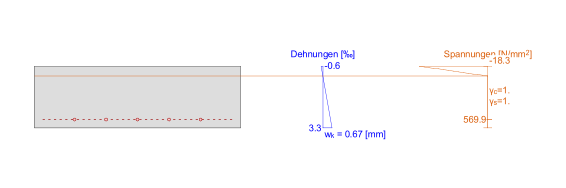
\includegraphics{A1_Traegerrost_Marti_files/mediabag/../imgs/jag_gerissene_steifigkeit_bearb.pdf}

}

\caption{\label{fig-jag_gerissene_steifigkeit}Querschnittsanalyse
Fliessen der Zugbewehrung, Beton völlig elastisch}

\end{figure}%

\[
\begin{aligned}
n& = \frac{E_{s , A}}{E_{c}} = 7.0 \  \quad &  \quad &  
 \end{aligned}
\]

Die Druckzonenhöhe wird mittels dem Gleichgewicht der horizontalen
Kräfte ermittelt

\[
\begin{aligned}
x_{II}& = 47.91 \ \mathrm{mm} \quad &  \quad &  
 \end{aligned}
\]

Damit lässt sich das Flächenträgheitsmoment bestimmen für den gerissenen
Querschnitt:

\[
\begin{aligned}
I_{cII}& = \frac{b_{w} \cdot x_{II}^{3}}{12} + b_{w} \cdot x_{II} \cdot \left(\frac{x_{II}}{2}\right)^{2} = 36650532.72 \ \mathrm{mm}^{4} \\ 
I_{sII}& = a_{s} \cdot b_{w} \cdot n \cdot \left(d_{x} - x_{II}\right)^{2} = 244534349.46 \ \mathrm{mm}^{4} \\ 
I_{II}& = I_{cII} + I_{sII} = 281184882.18 \ \mathrm{mm}^{4} \end{aligned}
\]

Abschliessend folgt die gerissene Biegesteifigkeit zu:

\[
\begin{aligned}
EI_{II , A}& = E_{c} \cdot I_{II} = 8238.72 \ \mathrm{kN} \cdot \mathrm{m}^{2} \quad &  \quad &  
 \end{aligned}
\]

\subsection{Hebelarm der inneren
Kräfte}\label{hebelarm-der-inneren-kruxe4fte}

Der Hebelarm der inneren Kräfte wird für den gesamten Träger als
konstant angenommen. Dabei wird dem Beton die Zylinderdruckfestigkeit
hinterlegt, sowie erreicht der Stahl die Zugfestigkeit.

\begin{figure}[H]

\centering{

\includegraphics{../imgs/jag_hebelarm_A.png}

}

\caption{\label{fig-jag_hebelarm_A}Querschnittsanalyse zur Bestimmung
des Hebelarms der inneren Kräfte}

\end{figure}%

\[
\begin{aligned}
x_{u , A}& = \frac{a_{s} \cdot b_{w} \cdot f_{su , A}}{0.85 \cdot b_{w} \cdot f_{cc}} = 18.11 \ \mathrm{mm} \\ 
z_{, A}& = d_{x} - 1 \cdot \frac{1}{2} \cdot 0.85 \cdot x_{u , A} = 253.3 \ \mathrm{mm} \\ 
m_{u , A}& = a_{s} \cdot f_{su , A} \cdot z_{, A} = 116.98 \ \frac{\mathrm{kNm}}{\mathrm{m}} \end{aligned}
\]

\subsection{Grenzzustände des
Zugglieds}\label{grenzzustuxe4nde-des-zugglieds}

Nun werden zwei Grenzzustände des Zugglieds betrachtet. Zum Einen bei
Fliessbeginn, zum anderen beim Erreichen der Zugfestigkeit. Dies dient
zur Ermittlung der mittleren Stahldehnung beim Erreichen eines
Fliessgelenks und einem plastischen Gelenk.

\subsubsection{\texorpdfstring{Risselement bei Fliessbeginn - Zustand
\(A1\)}{Risselement bei Fliessbeginn - Zustand A1}}\label{risselement-bei-fliessbeginn---zustand-a1}

Zunächst wird ein Grenzzustand betrachtet, bei dem das Risselement
gerade beim Fliessbeginn steht.

\[
\begin{aligned}
\sigma_{1 s , A1}& = f_{sy , A} = 570.0 \ \frac{\mathrm{N}}{\mathrm{mm}^{2}} \\ 
\sigma_{2 s , A1}& = f_{sy , A} - \frac{4 \cdot s_{r} \cdot \tau_{b0}}{2 \cdot \oslash_{x}} = 404.49 \ \frac{\mathrm{N}}{\mathrm{mm}^{2}} \end{aligned}
\]

Die folgenden Dehnungen stellen sich dabei ein:

\[
\begin{aligned}
\varepsilon_{1 s , A1}& = \frac{\sigma_{1 s , A1}}{E_{s , A}} = 2.78 \ \mathrm{‰} \\ 
\varepsilon_{2 s , A1}& = \frac{\sigma_{2 s , A1}}{E_{s , A}} = 1.97 \ \mathrm{‰} \end{aligned}
\]

Dabei stellt sich die folgende mittlere Stahldehnung ein. Berechnungen
nach {[}\citeproc{ref-marti_tragverhalten_1999}{4}{]} Seite 156.

\[
\begin{aligned}
\varepsilon_{m s , A1}& = 2.38 \ \mathrm{‰} \quad &  \quad &  
 \end{aligned}
\]

Das Fliessmoment beträgt dabei:

\[
\begin{aligned}
m_{y , A}& = a_{s} \cdot f_{sy , A} \cdot z_{, A} = 111.13 \ \frac{\mathrm{kNm}}{\mathrm{m}} \quad &  \quad &  
 \end{aligned}
\]

\begin{figure}[H]

\begin{minipage}{0.50\linewidth}

\centering{

\includegraphics{A1_Traegerrost_Marti_files/mediabag/../imgs/jag_stress_a1.pdf}

}

\subcaption{\label{fig-jag_stress_a1}Spannungsverlauf entlang des
Zugglieds auf halbem Rissabstand}

\end{minipage}%
%
\begin{minipage}{0.50\linewidth}

\centering{

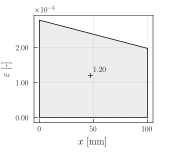
\includegraphics{A1_Traegerrost_Marti_files/mediabag/../imgs/jag_strain_a1.pdf}

}

\subcaption{\label{fig-jag_strain_a1}Dehnungsverlauf entlang des
Zugglieds auf halbem Rissabstand}

\end{minipage}%

\caption{\label{fig-jag_zustand_a1}Spannungs- und Dehnungsverlauf
entlang der Hälfte des Rissabstands für den Zustand \(A1\)}

\end{figure}%

\subsubsection{\texorpdfstring{Risselement beim Erreichen der
Zugfestigkeit - Zustand
\(A2\)}{Risselement beim Erreichen der Zugfestigkeit - Zustand A2}}\label{risselement-beim-erreichen-der-zugfestigkeit---zustand-a2}

Innerhalb des Risselements befindet sich der Betonstahl über der
Fliessgrenze, sowohl bereichsweise unterhalb der Fliessgrenze. Dies
führt zu den folgenden Spannungs- und Dehnungsverteilungen.

Dazu wird zunächst der Bereich bestimmt, in dem die Bewehrung sich im
plastischen Bereich befindet innerhalb des Zugglieds:

\[
\begin{aligned}
\Delta_{x pl , A2}& = \frac{f_{su , A} - f_{sy , A}}{4 \cdot \frac{1}{\oslash_{x}} \cdot \tau_{b1}} = 36.25 \ \mathrm{mm} \\ 
\Delta_{x el , A2}& = - \Delta_{x pl , A2} + \frac{s_{r}}{2} = 63.75 \ \mathrm{mm} \end{aligned}
\]

Die entsprechenden Spannungen und Dehnungen sin die folgenden.
Dargestellt sind diese in der Abbildung~\ref{fig-jag_zustand_a2}.

\[
\begin{aligned}
\sigma_{3 s , A2}& = - \frac{4 \cdot \Delta_{x el , A2} \cdot \tau_{b0}}{\oslash_{x}} + f_{sy , A} = 464.49 \ \frac{\mathrm{N}}{\mathrm{mm}^{2}} \\ 
\sigma_{2 s , A2}& = f_{sy , A} = 570.0 \ \frac{\mathrm{N}}{\mathrm{mm}^{2}} \\ 
\sigma_{1 s , A2}& = \frac{4 \cdot \Delta_{x pl , A2} \cdot \tau_{b1}}{\oslash_{x}} + f_{sy , A} = 600.0 \ \frac{\mathrm{N}}{\mathrm{mm}^{2}} \end{aligned}
\]

Die folgenden Dehnungen resultieren daraus:

\[
\begin{aligned}
\varepsilon_{1 s , A2}& = \varepsilon_{su , A} = 25 \ \mathrm{‰} \\ 
\varepsilon_{2 s , A2}& = \varepsilon_{sy , A} = 2.78 \ \mathrm{‰} \\ 
\varepsilon_{3 s , A2}& = \frac{\sigma_{3 s , A2}}{E_{s , A}} = 2.27 \ \mathrm{‰} \end{aligned}
\]

Und die mittlere Stahldehnung beträgt dabei:

\[
\begin{aligned}
\varepsilon_{m s , A2}& = 6.64 \ \mathrm{‰} \quad &  \quad &  
 \end{aligned}
\]

\begin{figure}[H]

\begin{minipage}{0.50\linewidth}

\centering{

\includegraphics{A1_Traegerrost_Marti_files/mediabag/../imgs/jag_stress_a2.pdf}

}

\subcaption{\label{fig-jag_stress_a2}Spannungsverlauf entlang des
Zugglieds auf halbem Rissabstand}

\end{minipage}%
%
\begin{minipage}{0.50\linewidth}

\centering{

\includegraphics{A1_Traegerrost_Marti_files/mediabag/../imgs/jag_strain_a2.pdf}

}

\subcaption{\label{fig-jag_strain_a2}Dehnungsverlauf entlang des
Zugglieds auf halbem Rissabstand}

\end{minipage}%

\caption{\label{fig-jag_zustand_a2}Spannungs- und Dehnungsverlauf
entlang der Hälfte des Rissabstands für den Zustand \(A2\)}

\end{figure}%

\subsubsection{Zusammenfassung}\label{zusammenfassung}

Zusammenfassend sind die Werte erneut aufgezeigt. Fliessen und Erreichen
der Zugfestigkeit:

\[
\begin{aligned}
\varepsilon_{m s , A1}& = 2.38 \ \mathrm{‰} \quad & m_{y , A}& = 111.13 \ \frac{\mathrm{kNm}}{\mathrm{m}} \\ 
\varepsilon_{m s , A2}& = 6.64 \ \mathrm{‰} \quad & m_{u , A}& = 116.98 \ \frac{\mathrm{kNm}}{\mathrm{m}} \end{aligned}
\]

\subsection{Systemanalyse}\label{systemanalyse}

Nun wird das System analysiert, sprich der Zweifeldträger.

\begin{figure}[H]

\centering{

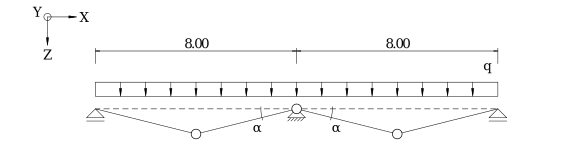
\includegraphics{A1_Traegerrost_Marti_files/mediabag/../imgs/jag_mechanismus.pdf}

}

\caption{\label{fig-jag_mechanismus}Definition der plastischen Rotation}

\end{figure}%

\begin{figure}[H]

\centering{

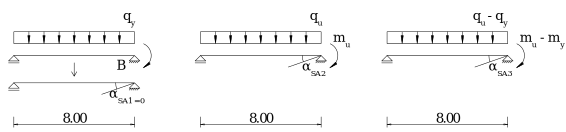
\includegraphics{A1_Traegerrost_Marti_files/mediabag/../imgs/jag_plast_rot_A.pdf}

}

\caption{\label{fig-jag_plast_rot_A}Definition der plastischen Rotation
beim Mittelauflager.Links ein Fliessen beim Mittelauflager führt zu
keiner plastischen Rotation, in der Mitte die maximale Rotation zum
Erreichen der Traglast, und rechts die effektive Traglast mit begrenzter
Plastischer Rotation}

\end{figure}%

\subsubsection{\texorpdfstring{Fliessen des Mittelauflagers - Zustand
\(SA1\)}{Fliessen des Mittelauflagers - Zustand SA1}}\label{fliessen-des-mittelauflagers---zustand-sa1}

Zunächst wird sich ein Fliessgelenk beim Mittelauflager ausbilden. Dazu
wird nun die zugehörige Streckenlast berechnet und die entsprechende
Felddeformation ermittelt.

\[
\begin{aligned}
m_{SA1 , B}& = m_{y , A} = 111.13 \ \frac{\mathrm{kNm}}{\mathrm{m}} \\ 
q_{SA1}& = \frac{8 \cdot b_{w} \cdot m_{SA1 , B}}{l^{2}} = 13.89 \ \frac{\mathrm{kN}}{\mathrm{m}} \\ 
w_{SA1}& = \frac{5 \cdot l^{4} \cdot q_{SA1}}{384 \cdot EI_{II , A}} - \frac{b_{w} \cdot l^{2} \cdot m_{y , A}}{16 \cdot EI_{II , A}} = 35.97 \ \mathrm{mm} \end{aligned}
\]

\subsubsection{\texorpdfstring{Fliessbeginn im Feld - Zustand
\(SA2\)}{Fliessbeginn im Feld - Zustand SA2}}\label{fliessbeginn-im-feld---zustand-sa2}

Beim Zustand zwei wird das Feldmoment ermittelt. Dabei wird beim
Mittelauflager der Biegewiderstand hinterlegt. Im Feld wird das
Fliessmoment angenommen.

\begin{figure}[H]

\centering{

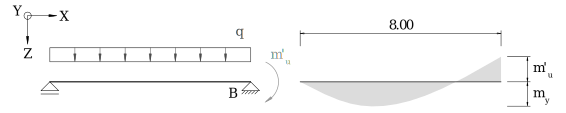
\includegraphics{A1_Traegerrost_Marti_files/mediabag/../imgs/jag_my_feld_A.pdf}

}

\caption{\label{fig-jag_my_feld_A}Fliessen im Feld}

\end{figure}%

Daraus lässt sich die entsprechende Streckenlast ermitteln. Dies bedingt
eine ausreichende Umlagerung, sprich Rotationsvermögen des
Mittelauflagers.

\[
\begin{aligned}
q_{SA2}& = b_{w} \cdot \left(\frac{2 \cdot m_{u , A} + 4 \cdot m_{y , A}}{l^{2}} + \frac{4 \cdot \sqrt{m_{u , A} \cdot m_{y , A} + m_{y , A}^{2}}}{l^{2}}\right) = 20.55 \ \frac{\mathrm{kN}}{\mathrm{m}} \end{aligned}
\]

\paragraph{Kontrolle der Duktilität}\label{kontrolle-der-duktilituxe4t}

Ob das Rotationsvermögen ausreichend ist, wird folglich bestimmt. Der
benötigte Rotationswinkel kann mithilfe der Arbeitsgleichung bestimmt
werden.

\[
\begin{aligned}
\alpha_{SA2}& = \frac{l^{3} \cdot \left(- q_{SA1} + q_{SA2}\right)}{24 \cdot EI_{II , A}} - \frac{b_{w} \cdot l \cdot \left(m_{u , A} - m_{y , A}\right)}{3 \cdot EI_{II , A}} = 0.88 \ \mathrm{°} \\ 
\Theta_{SA2 , erf}& = 2 \cdot \alpha_{SA2} = 1.76 \ \mathrm{°} \end{aligned}
\]

Der Plastische Roatationswinkel gibt die Rotation eines plastischen
Gelenks voraus.

\begin{figure}[H]

\centering{

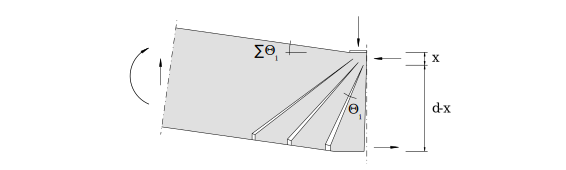
\includegraphics{A1_Traegerrost_Marti_files/mediabag/../imgs/jag_plast_gelenk.pdf}

}

\caption{\label{fig-plast_rot}Modell zur Abschätzung der plastischen
Rotation, nachgezeichnet nach {[}\citeproc{ref-kaufmann_2_2017}{5}{]}}

\end{figure}%

Dabei wird eine Länge des Gelenks angenommen, hier entspricht diese der
doppelten statischen Höhe. Für den Betonstahl B500A gilt daher die
folgende maximale plastische Roatation - sprich das Verformungsvermögen:

\[
\begin{aligned}
l_{pl}& = 2 \cdot d_{x} = 522.0 \ \mathrm{mm} \\ 
\Theta_{max , A}& = \frac{l_{pl} \cdot \left(- \varepsilon_{m s , A1} + \varepsilon_{m s , A2}\right)}{d_{x} - x_{u , A}} = 0.53 \ \mathrm{°} \end{aligned}
\]

Das Verformungsvermögen ist nicht ausreichend.

\subsubsection{\texorpdfstring{Ermittlung der Traglast - Zustand
\(SA3\)}{Ermittlung der Traglast - Zustand SA3}}\label{ermittlung-der-traglast---zustand-sa3}

Da das Verformungsvermögen nicht ausreicht, wird mittels dem
Verformungsvermögen die Traglast bestimmt. Dabei wird der
Rotationswinkel vorgegeben und die daraus resultierende Differenz der
Streckenlast zum Zustand \(SA1\) ermittelt. Aus der Addition der beiden
Zustände folgt die Traglast, welche das Verformungsvermögen einhält.

\[
\begin{aligned}
\alpha_{SA3}& = \frac{\Theta_{max , A}}{2} = 0.26 \ \mathrm{°} \\ 
\Delta_{q , SA3}& = \left(\alpha_{SA3} + \frac{b_{w} \cdot l \cdot \left(m_{u , A} - m_{y , A}\right)}{3 \cdot EI_{II , A}}\right) \cdot 24 \cdot EI_{II , A} \cdot \frac{1}{l^{3}} = 2.5 \ \frac{\mathrm{kN}}{\mathrm{m}} \\ 
q_{SA3}& = \Delta_{q , SA3} + q_{SA1} = 16.39 \ \frac{\mathrm{kN}}{\mathrm{m}} \end{aligned}
\]

Das Biegemoment im Feld stellt sich ein:

\[
\begin{aligned}
m_{SA3 , F}& = \frac{- \frac{b_{w} \cdot m_{u , A}}{2} + \frac{l^{2} \cdot q_{SA3}}{8} + \frac{\left(b_{w} \cdot m_{u , A}\right)^{2}}{2 \cdot l^{2} \cdot q_{SA3}}}{b_{w}} = 79.18 \ \frac{\mathrm{kNm}}{\mathrm{m}} \quad &  \quad &  
 \end{aligned}
\]

Dazu lässt sich für die Traglast ebenfalls die Felddurchbiegung
bestimmen.

\[
\begin{aligned}
w_{SA3}& = \frac{5 \cdot l^{4} \cdot q_{SA3}}{384 \cdot EI_{II , A}} - \frac{b_{w} \cdot l^{2} \cdot m_{u , A}}{16 \cdot EI_{II , A}} = 49.33 \ \mathrm{mm} \quad &  \quad &  
 \end{aligned}
\]

\subsubsection{Zusammenfassung}\label{zusammenfassung-1}

Abschliessend werden die zwei massgebenden Zustände kurz aufgegriffen.
Das Fliessen des Mittelauflagers erfolgt bei einer Streckenlast von
\(q_{SA1}\) und die Traglast entspricht \(q_{SA3}\).

\[
\begin{aligned}
q_{SA1}& = 13.89 \ \frac{\mathrm{kN}}{\mathrm{m}} \quad & w_{SA1}& = 35.97 \ \mathrm{mm} \quad & m_{SA1 , B}& = 111.13 \ \frac{\mathrm{kNm}}{\mathrm{m}} \\ 
q_{SA3}& = 16.39 \ \frac{\mathrm{kN}}{\mathrm{m}} \quad & w_{SA3}& = 49.33 \ \mathrm{mm} \quad & m_{SA3 , F}& = 79.18 \ \frac{\mathrm{kNm}}{\mathrm{m}} \end{aligned}
\]

\subsection{Federmodell}\label{federmodell}

Folgend wird das System mit dem Federmodell nachgerechnet.

\subsubsection{Momenten-Krümmungs-Beziehung}\label{momenten-kruxfcmmungs-beziehung}

Dazu wird eine Momenten-Krümmungs-Beziehung benötigt. Dabei wird das
Zuggurtmodell nicht berücksichtigt. Die entsprechenden Krümmungen werden
folgend berechnet:

\[
\begin{aligned}
EI_{II , A}& = E_{c} \cdot I_{II} = 8238.717 \ \mathrm{kN} \cdot \mathrm{m}^{2} \\ 
\chi_{y , A}& = \frac{b_{w} \cdot m_{y , A}}{EI_{II , A}} = 0.013 \ \frac{1}{\mathrm{m}} \\ 
\chi_{u , A}& = \frac{\varepsilon_{1 s , A2}}{d_{x} - x_{u , A}} = 0.103 \ \frac{1}{\mathrm{m}} \end{aligned}
\]

Mit den entsprechenden Biegemomenten

\[
\begin{aligned}
m_{y , A}& = a_{s} \cdot f_{sy , A} \cdot z_{, A} = 111.13 \ \frac{\mathrm{kNm}}{\mathrm{m}} \\ 
m_{u , A}& = a_{s} \cdot f_{su , A} \cdot z_{, A} = 116.98 \ \frac{\mathrm{kNm}}{\mathrm{m}} \end{aligned}
\]

Dargestellt ist dies in der Abbildung~\ref{fig-jag_m_chi_b500a}

\begin{figure}[H]

\centering{

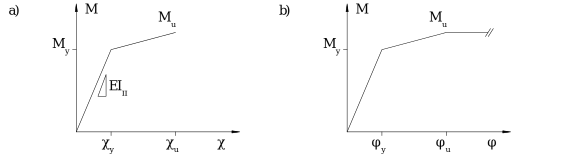
\includegraphics{A1_Traegerrost_Marti_files/mediabag/../imgs/jag_m_chi_b500a.pdf}

}

\caption{\label{fig-jag_m_chi_b500a}Momenten-Krümmungs-Beziehung
approximiert mit punktueller Querschnittsanalyse}

\end{figure}%

\subsubsection{Modellierung}\label{modellierung}

Die Elementlänge der starren Stäbe im Federmodell:

\[
\begin{aligned}
l_{El}& = 0.1 \ \mathrm{m} \quad &  \quad &  
 \end{aligned}
\]

Damit lässt sich die Fliessverdrehung und Bruchverdrehung definieren.

\[
\begin{aligned}
\Theta_{y , A}& = \chi_{y , A} \cdot l_{El} = 0.00135 \ \mathrm{rad} \\ 
\Theta_{u , A}& = \chi_{u , A} \cdot l_{El} = 0.01029 \ \mathrm{rad} \end{aligned}
\]

\subsubsection{Resultate}\label{resultate}

Abschliessend sind die Rotationen der Gelenke im Modell händisch zu
kontrollieren.

\paragraph{\texorpdfstring{Zustand
\(SA1\)}{Zustand SA1}}\label{zustand-sa1}

\[
\begin{aligned}
q_{SA1}& = 13.89 \ \frac{\mathrm{kN}}{\mathrm{m}} \quad &  \quad &  
 \end{aligned}
\]

\begin{figure}[H]

\centering{

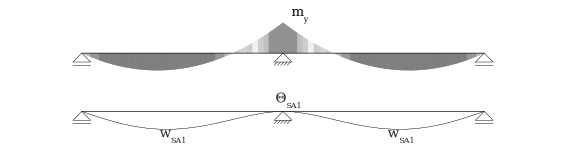
\includegraphics{A1_Traegerrost_Marti_files/mediabag/../imgs/jag_fem_sa1.pdf}

}

\caption{\label{fig-jag_fem_sa1}Verlauf der Biegemomente und
Deformationen für den Zustand \(SA1\), dazu die Stelle des
Rotationswinkels. Numerisch berechnet mit AxisVM Federmodell für den
Betonstahl B500A}

\end{figure}%

\[
\begin{aligned}
w_{SA1 , FEM}& = 37.4 \ \mathrm{mm} \quad & w_{SA1}& = 35.97 \ \mathrm{mm} \quad &  
 \end{aligned}
\]

\paragraph{\texorpdfstring{Zustand
\(SA3\)}{Zustand SA3}}\label{zustand-sa3}

\[
\begin{aligned}
q_{SA3}& = 16.39 \ \frac{\mathrm{kN}}{\mathrm{m}} \quad & m_{SA3 , F}& = 79.18 \ \frac{\mathrm{kNm}}{\mathrm{m}} \quad &  
 \end{aligned}
\]

\begin{figure}[H]

\centering{

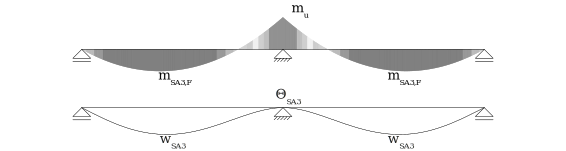
\includegraphics{A1_Traegerrost_Marti_files/mediabag/../imgs/jag_fem_sa3.pdf}

}

\caption{\label{fig-jag_feder_my_SA3}Verlauf der Biegemomente und
Deformationen für den Zustand \(SA3\), dazu die Stelle des
Rotationswinkels. Numerisch berechnet mit AxisVM Federmodell für den
Betonstahl B500A}

\end{figure}%

\[
\begin{aligned}
\Theta_{SA3 , FEM}& = 0.0092 \ \mathrm{rad} \quad & \Theta_{SA3}& = 0.0092 \ \mathrm{rad} \\ 
w_{SA3 , FEM}& = 50.5 \ \mathrm{mm} \quad & w_{SA3}& = 49.3262 \ \mathrm{mm} \end{aligned}
\]

\section{Naturharter Stahl B500C}\label{naturharter-stahl-b500c}

\subsection{Eigenschaften des
Betonstahls}\label{eigenschaften-des-betonstahls-1}

\[
\begin{aligned}
f_{sy , C}& = 500.0 \ \frac{\mathrm{N}}{\mathrm{mm}^{2}} \quad & f_{su , C}& = 600.0 \ \frac{\mathrm{N}}{\mathrm{mm}^{2}} \quad & \varepsilon_{sy , C}& = 2.44 \ \mathrm{‰} \\ 
\varepsilon_{sh , C}& = 20 \ \mathrm{‰} \quad & \varepsilon_{su , C}& = 125 \ \mathrm{‰} \quad & E_{s , C}& = 205.0 \ \frac{\mathrm{kN}}{\mathrm{mm}^{2}} \\ 
E_{sh , C}& = 952.0 \ \frac{\mathrm{N}}{\mathrm{mm}^{2}} \quad &  \quad &  
 \end{aligned}
\]

\begin{figure}[H]

{\centering 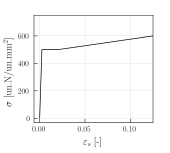
\includegraphics{A1_Traegerrost_Marti_files/mediabag/../imgs/jag_stress_strain_b500c.pdf}

}

\caption{Spannungs-Dehnungs-Beziehung des Betonstahls B500C}

\end{figure}%

\subsection{Linear elastische - gerissene
Biegesteifigkeit}\label{linear-elastische---gerissene-biegesteifigkeit-1}

Die Querschnittsanalyse wird von der Berechnung des kaltverformten
Betonstahls übernommen. Siehe
Abbildung~\ref{fig-jag_gerissene_steifigkeit}.

\[
\begin{aligned}
EI_{II , C}& = EI_{II , A} = 8238.72 \ \mathrm{kN} \cdot \mathrm{m}^{2} \\ 
x_{u , C}& = x_{u , A} = 18.11 \ \mathrm{mm} \\ 
z_{, C}& = z_{, A} = 253.3 \ \mathrm{mm} \end{aligned}
\]

\subsection{Gernzzustände des
Zugglieds}\label{gernzzustuxe4nde-des-zugglieds}

\subsubsection{\texorpdfstring{Risselement bei Fliessbeginn - Zustand
\(C1\)}{Risselement bei Fliessbeginn - Zustand C1}}\label{risselement-bei-fliessbeginn---zustand-c1}

Hier wird ein Zugglied analysiert, bei dem die Bewehrung die
Fliessspannung erreicht. Dabei stellen sich folgende Spannungen entlang
dem Risselement ein:

\[
\begin{aligned}
\sigma_{1 s , C1}& = f_{sy , C} = 500.0 \ \frac{\mathrm{N}}{\mathrm{mm}^{2}} \\ 
\sigma_{2 s , C1}& = f_{sy , C} - \frac{4 \cdot s_{r} \cdot \tau_{b0}}{2 \cdot \oslash_{x}} = 334.49 \ \frac{\mathrm{N}}{\mathrm{mm}^{2}} \end{aligned}
\]

Und die folgenden Dehnungen stellen sich ein:

\[
\begin{aligned}
\varepsilon_{1 s , C1}& = \frac{\sigma_{1 s , C1}}{E_{s , C}} = 2.44 \ \mathrm{‰} \\ 
\varepsilon_{2 s , C1}& = \frac{\sigma_{2 s , C1}}{E_{s , C}} = 1.63 \ \mathrm{‰} \end{aligned}
\]

Die Mittlere Dehnung ist die folgende. Diese gilt es nach
{[}\citeproc{ref-alvarez_einfluss_1998}{6}{]} Seite 163 zu bestimmen.

\[
\begin{aligned}
\varepsilon_{m s , C1}& = 2.04 \ \mathrm{‰} \quad &  \quad &  
 \end{aligned}
\]

\[
\begin{aligned}
m_{y , C}& = a_{s} \cdot f_{sy , C} \cdot z_{, C} = 97.48 \ \frac{\mathrm{kNm}}{\mathrm{m}} \quad &  \quad &  
 \end{aligned}
\]

\begin{figure}[H]

\begin{minipage}{0.50\linewidth}

\centering{

\includegraphics{A1_Traegerrost_Marti_files/mediabag/../imgs/jag_stress_c1.pdf}

}

\subcaption{\label{fig-jag_stress_c1}Spannungsverlauf entlang des
Zugglieds auf halbem Rissabstand}

\end{minipage}%
%
\begin{minipage}{0.50\linewidth}

\centering{

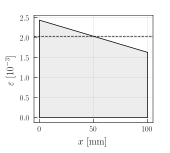
\includegraphics{A1_Traegerrost_Marti_files/mediabag/../imgs/jag_strain_c1.pdf}

}

\subcaption{\label{fig-jag_strain_c1}Dehnungsverlauf entlang des
Zugglieds auf halbem Rissabstand}

\end{minipage}%

\caption{\label{fig-jag_zustand_c1}Spannungs- und Dehnungsverlauf
entlang der Hälfte des Rissabstands für den Zustand \(C1\)}

\end{figure}%

\subsubsection{\texorpdfstring{Risselement beim Erreichen der
Zugfestigkeit - Zustand
\(C2\)}{Risselement beim Erreichen der Zugfestigkeit - Zustand C2}}\label{risselement-beim-erreichen-der-zugfestigkeit---zustand-c2}

Innerhalb des Risselements befindet sich der Betonstahl über der
Fliessgrenze. Dies führt zu den folgenden Spannungs- und
Dehnungsverteilungen.

\[
\begin{aligned}
\sigma_{1 s , C2}& = f_{su , C} = 600.0 \ \frac{\mathrm{N}}{\mathrm{mm}^{2}} \\ 
\sigma_{2 s , C2}& = f_{su , C} - \frac{4 \cdot s_{r} \cdot \tau_{b1}}{2 \cdot \oslash_{x}} = 517.24 \ \frac{\mathrm{N}}{\mathrm{mm}^{2}} \end{aligned}
\]

Die Dehnungen sind die folgenden:

\[
\begin{aligned}
\varepsilon_{1 s , C2}& = \varepsilon_{sh , C} + \frac{- f_{sy , C} + \sigma_{2 s , C2}}{E_{sh , C}} = 38.11 \ \mathrm{‰} \\ 
\varepsilon_{2 s , C2}& = \varepsilon_{su , C} = 125 \ \mathrm{‰} \end{aligned}
\]

Und die mittlere Stahldehnung beträgt dabei:

\[
\begin{aligned}
\varepsilon_{m s , C2}& = 81.56 \ \mathrm{‰} \quad &  \quad &  
 \end{aligned}
\]

Kontrolliert wird die Betonstauchung. Es zeigt sich, dass sich ein
Betondruckversagen einstellt. Die Betonbruchstauchung basiert auf einem
Erfahrungswert.

\[
\begin{aligned}
\varepsilon_{c , C2}& = 6.08 \ \mathrm{‰} \quad & \varepsilon_{cu}& = 5 \ \mathrm{‰} \quad &  
 \end{aligned}
\]

Die zulässige mittlere Stahldehnung beträgt folglich:

\[
\begin{aligned}
\varepsilon_{m s , adm}& = \frac{\varepsilon_{cu} \cdot \left(d_{x} - x_{u , C}\right)}{x_{u , C}} = 67.06 \ \mathrm{‰} \quad &  \quad &  
 \end{aligned}
\]

Damit folgen die Dehnungen für diesen Zustand zu:

\[
\begin{aligned}
\varepsilon_{1 s , C2}& = \tau_{b1} \cdot 4 \cdot s_{r} \cdot \frac{1}{4} \cdot \frac{1}{E_{sh , C} \cdot \oslash_{x}} + \varepsilon_{m s , adm} = 110.52 \ \mathrm{‰} \\ 
\varepsilon_{2 s , C2}& = - \frac{4 \cdot s_{r} \cdot \tau_{b1}}{4 \cdot E_{sh , C} \cdot \oslash_{x}} + \varepsilon_{m s , adm} = 23.59 \ \mathrm{‰} \end{aligned}
\]

Und daraus werden die Spannungen bestimmt:

\[
\begin{aligned}
\sigma_{1 s , C2}& = E_{sh , C} \cdot \left(\varepsilon_{1 s , C2} - \varepsilon_{sh , C}\right) + f_{sy , C} = 586.18 \ \frac{\mathrm{N}}{\mathrm{mm}^{2}} \\ 
\sigma_{2 s , C2}& = E_{sh , C} \cdot \left(\varepsilon_{2 s , C2} - \varepsilon_{sh , C}\right) + f_{sy , C} = 503.42 \ \frac{\mathrm{N}}{\mathrm{mm}^{2}} \end{aligned}
\]

Dabei folgt der Biegewiderstand, begrenzt durch ein Betondruckversagen,
zu:

\[
\begin{aligned}
m_{u , C}& = a_{s} \cdot \sigma_{1 s , C2} \cdot z_{, C} = 114.28 \ \frac{\mathrm{kNm}}{\mathrm{m}} \quad &  \quad &  
 \end{aligned}
\]

\begin{figure}[H]

\begin{minipage}{0.50\linewidth}

\centering{

\includegraphics{A1_Traegerrost_Marti_files/mediabag/../imgs/jag_stress_c2.pdf}

}

\subcaption{\label{fig-jag_stress_c2}Spannungsverlauf entlang des
Zugglieds auf halbem Rissabstand}

\end{minipage}%
%
\begin{minipage}{0.50\linewidth}

\centering{

\includegraphics{A1_Traegerrost_Marti_files/mediabag/../imgs/jag_strain_c2.pdf}

}

\subcaption{\label{fig-jag_strain_c2}Dehnungsverlauf entlang des
Zugglieds auf halbem Rissabstand}

\end{minipage}%

\caption{\label{fig-jag_zustand_c2}Spannungs- und Dehnungsverlauf
entlang der Hälfte des Rissabstands für den Zustand \(C2\)}

\end{figure}%

\subsubsection{Zusammenfassung}\label{zusammenfassung-2}

Zusammenfassend sind die Werte erneut aufgezeigt. Fliessen und Erreichen
der Betonbruchstauchung:

\[
\begin{aligned}
\varepsilon_{m s , C1}& = 2.04 \ \mathrm{‰} \quad & m_{y , C}& = 97.48 \ \frac{\mathrm{kNm}}{\mathrm{m}} \\ 
\varepsilon_{m s , adm}& = 67.06 \ \mathrm{‰} \quad & m_{u , C}& = 114.28 \ \frac{\mathrm{kNm}}{\mathrm{m}} \end{aligned}
\]

\subsection{Systemanalyse}\label{systemanalyse-1}

Nun wird das System analysiert, sprich der Zweifeldträger. Siehe
Abbildung~\ref{fig-jag_mechanismus} und
Abbildung~\ref{fig-jag_plast_rot_A}.

\subsubsection{\texorpdfstring{Fliessen des Mittelauflager - Zustand
\(SC1\)}{Fliessen des Mittelauflager - Zustand SC1}}\label{fliessen-des-mittelauflager---zustand-sc1}

Auch hier stellt sich zunächst ein Fliessgelenk beim Mittelauflager ein.
Dazu wird nun diezugehörige Streckenlast berechnet und die entsprechende
Felddeformation ermittelt.

\[
\begin{aligned}
m_{SC1 , B}& = m_{y , C} = 97.48 \ \frac{\mathrm{kNm}}{\mathrm{m}} \\ 
q_{SC1}& = \frac{8 \cdot b_{w} \cdot m_{SC1 , B}}{l^{2}} = 12.19 \ \frac{\mathrm{kN}}{\mathrm{m}} \\ 
w_{SC1}& = \frac{5 \cdot l^{4} \cdot q_{SC1}}{384 \cdot EI_{II , C}} - \frac{b_{w} \cdot l^{2} \cdot m_{SC1 , B}}{16 \cdot EI_{II , C}} = 31.55 \ \mathrm{mm} \end{aligned}
\]

\[
\begin{aligned}
\Theta_{max , C}& = \frac{l_{pl} \cdot \left(- \varepsilon_{m s , C1} + \varepsilon_{m s , adm}\right)}{d_{x} - x_{u , C}} = 8.01 \ \mathrm{°} \quad &  \quad &  
 \end{aligned}
\]

\subsubsection{\texorpdfstring{Fliessbeginn im Feld - Zustand
\(SC2\)}{Fliessbeginn im Feld - Zustand SC2}}\label{fliessbeginn-im-feld---zustand-sc2}

Beim Zustand zwei wird das Feldmoment ermittelt. Dabei wird beim
Mittelauflager der Biegewiderstand hinterlegt. Dem Feld wird das
Fliessmoment vorausgesetzt. Siehe dazu
Abbildung~\ref{fig-jag_my_feld_A}.

\[
\begin{aligned}
m_{SC2 , F}& = m_{y , C} = 97.48 \ \frac{\mathrm{kNm}}{\mathrm{m}} \quad &  \quad &  
 \end{aligned}
\]

Das Biegemoment im Feld wird anhand der plastischen Rotation bestimmt.
Siehe dazu Abbildung~\ref{fig-jag_plast_rot_A}. Dabei werden die
Spannungen und Dehnungen innerhalb des Zugglieds bestimmt. Dabei
betragen die Spannungen:

\[
\begin{aligned}
\Delta_{x pl , SC2}& = \Delta_{x pl , A2} = 36.25 \ \mathrm{mm} \\ 
\Delta_{x el , SC2}& = - \Delta_{x pl , SC2} + \frac{s_{r}}{2} = 63.75 \ \mathrm{mm} \end{aligned}
\]

\[
\begin{aligned}
\sigma_{2 s , SC2}& = 500 = 500.0 \ \frac{\mathrm{N}}{\mathrm{mm}^{2}} \\ 
\sigma_{1 s , SC2}& = \frac{4 \cdot \Delta_{x pl , SC2} \cdot \tau_{b1}}{\oslash_{x}} + \sigma_{2 s , SC2} = 530.0 \ \frac{\mathrm{N}}{\mathrm{mm}^{2}} \\ 
\sigma_{3 s , SC2}& = - \frac{4 \cdot \Delta_{x el , SC2} \cdot \tau_{b0}}{\oslash_{x}} + \sigma_{2 s , SC2} = 394.49 \ \frac{\mathrm{N}}{\mathrm{mm}^{2}} \end{aligned}
\]

Und die Dehnungen definieren sich zu:

\[
\begin{aligned}
\varepsilon_{1 s , SC2}& = \varepsilon_{sh , C} + \frac{\sigma_{1 s , SC2} - \sigma_{2 s , SC2}}{E_{sh , C}} = 51.51 \ \mathrm{‰} \\ 
\varepsilon_{21 s , SC2}& = \varepsilon_{sh , C} = 20 \ \mathrm{‰} \\ 
\varepsilon_{22 s , SC2}& = \varepsilon_{sy , A} = 2.78 \ \mathrm{‰} \\ 
\varepsilon_{3 s , SC2}& = \frac{\sigma_{3 s , SC2}}{E_{s , A}} = 1.92 \ \mathrm{‰} \end{aligned}
\]

Abschliessend lässt sich für die trilineare Spannungs-Dehnungs-Beziehung
die Mittlere Dehnung bestimmen. Diese gilt es nach
{[}\citeproc{ref-alvarez_einfluss_1998}{6}{]} Seite 163 zu bestimmen,
wurde in diesem Beispiel jedoch vom Skript
{[}\citeproc{ref-jager_stahlbeton_2009}{2}{]} übernommen.

\[
\begin{aligned}
\varepsilon_{m s , SC2}& = 14.33 \ \mathrm{‰} \end{aligned}
\]

Dargestellt sind die Resultate in der
Abbildung~\ref{fig-jag_zustand_sc2}.

\begin{figure}[H]

\begin{minipage}{0.50\linewidth}

\centering{

\includegraphics{A1_Traegerrost_Marti_files/mediabag/../imgs/jag_stress_sc2.pdf}

}

\subcaption{\label{fig-jag_stress_sc2}Spannungsverlauf entlang des
Zugglieds auf halbem Rissabstand}

\end{minipage}%
%
\begin{minipage}{0.50\linewidth}

\centering{

\includegraphics{A1_Traegerrost_Marti_files/mediabag/../imgs/jag_strain_sc2.pdf}

}

\subcaption{\label{fig-jag_strain_sc2}Dehnungsverlauf entlang des
Zugglieds auf halbem Rissabstand}

\end{minipage}%

\caption{\label{fig-jag_zustand_sc2}Spannungs- und Dehnungsverlauf
entlang der Hälfte des Rissabstands für den Zustand \(SC2\)}

\end{figure}%

Dabei stellt sich das folgende plastische Rotationsvermögen ein:

\[
\begin{aligned}
\Theta_{SC2 , pl}& = \frac{l_{pl} \cdot \left(- \varepsilon_{m s , C1} + \varepsilon_{m s , SC2}\right)}{d_{x} - x_{u , C}} = 1.51 \ \mathrm{°} \quad &  \quad &  
 \end{aligned}
\]

Anhand dieses Zustands können Streckenlast und Feldmoment bestimmt
werden:

\[
\begin{aligned}
m_{SC2 , B}& = a_{s} \cdot \sigma_{1 s , SC2} \cdot z_{, A} = 103.33 \ \frac{\mathrm{kNm}}{\mathrm{m}} \quad &  \quad &  
 \end{aligned}
\]

\[
\begin{aligned}
q_{SC2}& = b_{w} \cdot \left(\frac{2 \cdot m_{SC2 , F} + 4 \cdot m_{y , C}}{l^{2}} + \frac{4 \cdot \sqrt{m_{SC2 , B} \cdot m_{SC2 , F} + m_{SC2 , F}^{2}}}{l^{2}}\right) = 17.88 \ \frac{\mathrm{kN}}{\mathrm{m}} \end{aligned}
\]

Dabei wird nun kontrolliert, ob das Rotationsvermögen ausreichend ist
für den Rotationsbedarf. Der Rotationsbedarf beträgt dabei:

\[
\begin{aligned}
\alpha_{SC2}& = \frac{l^{3} \cdot \left(- q_{SC1} + q_{SC2}\right)}{24 \cdot EI_{II , C}} - \frac{b_{w} \cdot l \cdot \left(m_{SC2 , B} - m_{SC2 , F}\right)}{3 \cdot EI_{II , C}} = 0.74 \ \mathrm{°} \\ 
\Theta_{SC2 , erf}& = 2 \cdot \alpha_{SC2} = 1.47 \ \mathrm{°} \\ 
\Delta_{\Theta SC3}& = \Theta_{SC2 , erf} - \Theta_{SC2 , pl} = -0.04 \ \mathrm{°} \end{aligned}
\]

Es ist folglich ein gültiger Zustand gefunden worden. Dies ist iterativ
zu bestimmen. Die entsprechende Deformation im Feld beträgt dabei:

\[
\begin{aligned}
w_{SC2}& = \frac{5 \cdot l^{4} \cdot q_{SC2}}{384 \cdot EI_{II , A}} - \frac{b_{w} \cdot l^{2} \cdot m_{SC2 , B}}{16 \cdot EI_{II , A}} = 65.6 \ \mathrm{mm} \quad &  \quad &  
 \end{aligned}
\]

\subsubsection{\texorpdfstring{Ermittlung der Traglast - Zustand
\(SC3\)}{Ermittlung der Traglast - Zustand SC3}}\label{ermittlung-der-traglast---zustand-sc3}

Da die maximale plastische Rotation noch nicht erreicht worden ist,
lässt sich die Last weiter steigern. Dazu wird ein Zustand gesucht,
welcher eine Rotation beim Mittelauflager hervorruft, welche der
maximalen plastischen Rotation entspricht. Dabei werden folgende
Dehnungen im Risselement angenommen:

\[
\begin{aligned}
\varepsilon_{2 s , SC3}& = \varepsilon_{sh , C} = 20 \ \mathrm{‰} \\ 
\varepsilon_{1 s , SC3}& = \frac{4 \cdot s_{r} \cdot \tau_{b1}}{2 \cdot E_{sh , C} \cdot \oslash_{x}} + \varepsilon_{2 s , SC3} = 106.93 \ \mathrm{‰} \\ 
\varepsilon_{m s , SC3}& = \frac{\varepsilon_{1 s , SC3} + \varepsilon_{2 s , SC3}}{2} = 63.46 \ \mathrm{‰} \end{aligned}
\]

Dabei stellen sich folgende Spannungen ein:

\[
\begin{aligned}
\sigma_{1 s , SC3}& = E_{sh , C} \cdot \left(\varepsilon_{1 s , SC3} - \varepsilon_{2 s , SC3}\right) + f_{sy , C} = 582.76 \ \frac{\mathrm{N}}{\mathrm{mm}^{2}} \\ 
\sigma_{2 s , SC3}& = f_{sy , C} = 500.0 \ \frac{\mathrm{N}}{\mathrm{mm}^{2}} \end{aligned}
\]

Dargestellt ist dies in der Abbildung~\ref{fig-jag_zustand_sc3}.

\begin{figure}[H]

\begin{minipage}{0.50\linewidth}

\centering{

\includegraphics{A1_Traegerrost_Marti_files/mediabag/../imgs/jag_stress_sc3.pdf}

}

\subcaption{\label{fig-jag_stress_sc3}Spannungsverlauf entlang des
Zugglieds auf halbem Rissabstand}

\end{minipage}%
%
\begin{minipage}{0.50\linewidth}

\centering{

\includegraphics{A1_Traegerrost_Marti_files/mediabag/../imgs/jag_strain_sc3.pdf}

}

\subcaption{\label{fig-jag_strain_sc3}Dehnungsverlauf entlang des
Zugglieds auf halbem Rissabstand}

\end{minipage}%

\caption{\label{fig-jag_zustand_sc3}Spannungs- und Dehnungsverlauf
entlang der Hälfte des Rissabstands für die Traglast}

\end{figure}%

Mit der gewählten Rotation stellt sich das folgende Feldmoment ein:

\[
\begin{aligned}
m_{SC3 , F}& = a_{s} \cdot \sigma_{1 s , SC3} \cdot z_{, C} = 113.62 \ \frac{\mathrm{kNm}}{\mathrm{m}} \\ 
m_{SC3 , B}& = m_{u , C} = 114.28 \ \frac{\mathrm{kNm}}{\mathrm{m}} \end{aligned}
\]

Und die dazu entsprechende Streckenlast:

\[
\begin{aligned}
q_{SC3}& = b_{w} \cdot \left(\frac{4 \cdot m_{SC3 , F} + 2 \cdot m_{u , C}}{l^{2}} + \frac{4 \cdot \sqrt{m_{SC3 , F}^{2} + m_{SC3 , F} \cdot m_{u , C}}}{l^{2}}\right) = 20.73 \ \frac{\mathrm{kN}}{\mathrm{m}} \quad &  \quad &  
 \end{aligned}
\]

Dabei ist nun die plastische Rotation im Feld zu kontrollieren. Dabei
ist die Lage des Gelenks abzuschätzen. Dabei entspricht \(w\) der
plastischen Rotation, welche kleiner als das Rotationsvermögen sein
muss.

\begin{figure}[H]

\centering{

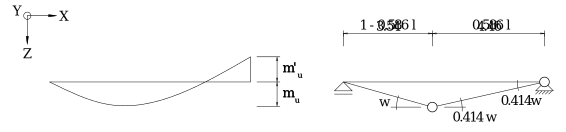
\includegraphics{A1_Traegerrost_Marti_files/mediabag/../imgs/jag_plast_feld_C.pdf}

}

\caption{\label{fig-jag_plast_feld_C}Annahme für die Lage des Gelenks im
Feld}

\end{figure}%

Dabei stellt sich die folgende plastische Rotation im Feld ein:

\[
\begin{aligned}
\Theta_{SC3 , F}& = \frac{l_{pl} \cdot \left(- \varepsilon_{m s , C1} + \varepsilon_{m s , SC3}\right)}{d_{x} - x_{u , A}} = 7.56 \ \mathrm{°} \quad &  \quad &  
 \end{aligned}
\]

Und beim Mittelauflager muss die folgende Rotation verfügbar sein:

\[
\begin{aligned}
\alpha_{SC3}& = 0.414 \cdot \Theta_{SC3 , F} + \frac{l^{3} \cdot q_{SC3}}{24 \cdot EI_{II , A}} - \frac{b_{w} \cdot l \cdot m_{u , C}}{3 \cdot EI_{II , A}} = 4.09 \ \mathrm{°} \\ 
\Theta_{SC3 , erf}& = 2 \cdot \alpha_{SC3} = 8.18 \ \mathrm{°} \end{aligned}
\]

Welche mit der maximalen plastischen Rotation zu vergleichen ist.

\[
\begin{aligned}
\Theta_{max , C}& = \frac{l_{pl} \cdot \left(- \varepsilon_{m s , C1} + \varepsilon_{m s , adm}\right)}{d_{x} - x_{u , C}} = 8.01 \ \mathrm{°} \\ 
\Delta_{\Theta SC3}& = \Theta_{SC3 , erf} - \Theta_{max , C} = 0.17 \ \mathrm{°} \end{aligned}
\]

Die erforderliche Rotation des Mittelauflagers ist in etwa gleich dem
Rotationsvermögen. Abschliessend stellt sich die folgende Feldverformung
ein:

\[
\begin{aligned}
w_{SC3}& = \frac{0.414 \cdot \Theta_{SC3 , F} \cdot l}{2} + \frac{5 \cdot l^{4} \cdot q_{SC3}}{384 \cdot EI_{II , C}} - \frac{b_{w} \cdot l^{2} \cdot m_{u , C}}{16 \cdot EI_{II , A}} = 297.33 \ \mathrm{mm} \quad &  \quad &  
 \end{aligned}
\]

\subsubsection{Zusammenfassung}\label{zusammenfassung-3}

\[
\begin{aligned}
q_{SC1}& = 12.19 \ \frac{\mathrm{kN}}{\mathrm{m}} \quad & w_{SC1}& = 31.55 \ \mathrm{mm} \quad & m_{SC1 , B}& = 97.48 \ \frac{\mathrm{kNm}}{\mathrm{m}} \\ 
q_{SC2}& = 17.88 \ \frac{\mathrm{kN}}{\mathrm{m}} \quad & w_{SC2}& = 65.6 \ \mathrm{mm} \quad & m_{SC2 , B}& = 103.33 \ \frac{\mathrm{kNm}}{\mathrm{m}} \\ 
q_{SC3}& = 20.73 \ \frac{\mathrm{kN}}{\mathrm{m}} \quad & w_{SC3}& = 297.33 \ \mathrm{mm} \quad & m_{SC3 , F}& = 113.62 \ \frac{\mathrm{kNm}}{\mathrm{m}} \end{aligned}
\]

\subsection{Federmodell}\label{federmodell-1}

\subsubsection{Momenten-Krümmungs-Beziehung}\label{momenten-kruxfcmmungs-beziehung-1}

Dabei lassen sich die folgenden Krümmungen bestimmen:

\[
\begin{aligned}
\chi_{y , C}& = \frac{b_{w} \cdot m_{y , C}}{EI_{II , C}} = 0.0118 \ \frac{1}{\mathrm{m}} \\ 
\chi_{sh , C}& = \frac{\varepsilon_{sh , C}}{d_{x} - x_{u , C}} = 0.0823 \ \frac{1}{\mathrm{m}} \\ 
\chi_{u , C}& = \frac{\varepsilon_{1 s , C2}}{d_{x} - x_{u , C}} = 0.455 \ \frac{1}{\mathrm{m}} \end{aligned}
\]

Mit den entsprechenden Biegemomenten:

\[
\begin{aligned}
m_{y , C}& = a_{s} \cdot f_{sy , C} \cdot z_{, C} = 97.48 \ \frac{\mathrm{kNm}}{\mathrm{m}} \\ 
m_{u , C}& = a_{s} \cdot \sigma_{1 s , C2} \cdot z_{, C} = 114.28 \ \frac{\mathrm{kNm}}{\mathrm{m}} \end{aligned}
\]

Aufgezeigt ist die Momenten-Krümmungs-Beziehung in der
Abbildung~\ref{fig-jag_m_chi_b500c}.

\begin{figure}[H]

\centering{

\includegraphics{A1_Traegerrost_Marti_files/mediabag/../imgs/jag_m_chi_b500c.pdf}

}

\caption{\label{fig-jag_m_chi_b500c}Momenten-Krümmungs-Beziehung
approximiert mit punktueller Querschnittsanalyse für den Betonstahl
B500C}

\end{figure}%

\subsubsection{Modellierung}\label{modellierung-1}

Die Elementlänge der starren Stäbe im Federmodell betragen:

\[
\begin{aligned}
l_{El}& = 0.1 \ \mathrm{m} \quad &  \quad &  
 \end{aligned}
\]

Damit lassen sich die Grenzpunkte der Krümmung in eine Verdrehung
umrechnen:

\[
\begin{aligned}
\Theta_{y , C}& = \chi_{y , C} \cdot l_{El} = 0.0011832 \ \mathrm{rad} \\ 
\Theta_{sh , C}& = \chi_{sh , C} \cdot l_{El} = 0.0082342 \ \mathrm{rad} \\ 
\Theta_{u , C}& = \chi_{u , C} \cdot l_{El} = 0.0455032 \ \mathrm{rad} \end{aligned}
\]

\subsubsection{Resultate}\label{resultate-1}

Abschliessend sind die Rotationen der Gelenke im Modell händisch zu
kontrollieren.

\paragraph{\texorpdfstring{Zustand
\(SC1\)}{Zustand SC1}}\label{zustand-sc1}

\[
\begin{aligned}
q_{SC1}& = 12.19 \ \frac{\mathrm{kN}}{\mathrm{m}} \quad &  \quad &  
 \end{aligned}
\]

\begin{figure}[H]

\centering{

\includegraphics{A1_Traegerrost_Marti_files/mediabag/../imgs/jag_fem_sa1.pdf}

}

\caption{\label{fig-jag_feder_my_SC1}Verlauf der Biegemomente und
Deformationen für den Zustand \(SA1\), dazu die Stelle des
Rotationswinkels. Numerisch berechnet mit AxisVM Federmodell für den
Betonstahl PLATZHALTER}

\end{figure}%

\[
\begin{aligned}
w_{SC1 , FEM}& = 32.0 \ \mathrm{mm} \quad & w_{SC1}& = 31.55 \ \mathrm{mm} \quad &  
 \end{aligned}
\]

\paragraph{\texorpdfstring{Zustand
\(SC2\)}{Zustand SC2}}\label{zustand-sc2}

\[
\begin{aligned}
q_{SC2}& = 17.88 \ \frac{\mathrm{kN}}{\mathrm{m}} \quad &  \quad &  
 \end{aligned}
\]

\begin{figure}[H]

\centering{

\includegraphics{A1_Traegerrost_Marti_files/mediabag/../imgs/jag_fem_sa1.pdf}

}

\caption{\label{fig-jag_feder_my_SC2}Verlauf der Biegemomente und
Deformationen für den Zustand \(SA2\), dazu die Stelle des
Rotationswinkels. Numerisch berechnet mit AxisVM Federmodell für den
Betonstahl PLATZHALTER}

\end{figure}%

\[
\begin{aligned}
w_{SC2 , FEM}& = 60.0 \ \mathrm{mm} \quad & w_{SC2}& = 65.6 \ \mathrm{mm} \quad &  
 \end{aligned}
\]

\paragraph{\texorpdfstring{Zustand
\(SC3\)}{Zustand SC3}}\label{zustand-sc3}

\[
\begin{aligned}
q_{SC3}& = 20.73 \ \frac{\mathrm{kN}}{\mathrm{m}} \quad & m_{SC3 , F}& = 113.62 \ \frac{\mathrm{kNm}}{\mathrm{m}} \quad & m_{SC3 , B}& = 114.28 \ \frac{\mathrm{kNm}}{\mathrm{m}} \end{aligned}
\]

\begin{figure}[H]

\centering{

\includegraphics{A1_Traegerrost_Marti_files/mediabag/../imgs/jag_fem_sa1.pdf}

}

\caption{\label{fig-jag_feder_my_SC2}Verlauf der Biegemomente und
Deformationen für den Zustand \(SA2\), dazu die Stelle des
Rotationswinkels. Numerisch berechnet mit AxisVM Federmodell für den
Betonstahl PLATZHALTER}

\end{figure}%

Die Lage des Gelenks:

\[
\begin{aligned}
x_{Gelenk , FEM}& = 3.3 \ \mathrm{m} \quad & x_{Gelenk}& = 3.31 \ \mathrm{m} \quad &  
 \end{aligned}
\]

\[
\begin{aligned}
q_{SC3 FEM}& = 18.9 \ \frac{\mathrm{kN}}{\mathrm{m}} \quad & w_{SC3 FEM}& = 229.08 \ \mathrm{mm} \quad & w_{SC3}& = 297.33 \ \mathrm{mm} \end{aligned}
\]

\section{Zusammenfassung der
Resultate}\label{zusammenfassung-der-resultate}

\begin{figure}[H]

\centering{

\includegraphics{A1_Traegerrost_Marti_files/mediabag/../imgs/jag_q_w.pdf}

}

\caption{\label{fig-jag_q_w}Last-Feldmittendurchbiegung-Diagramm für
beide Betonstähle, analytisch gelöst und mit der FEM-Lösung
nachgerechnet}

\end{figure}%

\chapter{Versuchsnachrechnung
Zweifeldplatte}\label{versuchsnachrechnung-zweifeldplatte}

Nachrechnung des Plattenversuchs aus
{[}\citeproc{ref-thoma_plattenversuche_2010}{7}{]}. Gleiche
Kraftintensität auf allen Zylindern. Eigengewicht hat keinen Einfluss
auf Messung, Nullsetzung bei Belastungsbeginn.

\begin{figure}[H]

\centering{

\includegraphics{A1_Traegerrost_Marti_files/mediabag/../imgs/tho_aufbau_iso.pdf}

}

\caption{\label{fig-tho_aufbau_iso}Isometrische Ansicht des
Versuchsaufbaus, dargestellt sind der Versuchsaufbau, die Lagerung mit
den Zylindern, die Krafteinleitung mittels den Zugstangen}

\end{figure}%

\begin{figure}[H]

\centering{

\includegraphics{A1_Traegerrost_Marti_files/mediabag/../imgs/tho_aufbau_gr.pdf}

}

\caption{\label{fig-tho_aufbau_gr}Grundriss und Längsansicht,
Lasteineinleitung, Lagerposition und die Plattenabmessungen sind
vermasst}

\end{figure}%

\section{Versuchsbeschrieb}\label{versuchsbeschrieb}

\subsection{Berechnungsgrössen}\label{berechnungsgruxf6ssen}

\subsubsection{Betonstahl}\label{betonstahl}

\begin{figure}[H]

\centering{

\includegraphics{A1_Traegerrost_Marti_files/mediabag/../imgs/tho_biegebewehrung_iso.pdf}

}

\caption{\label{fig-tho_biegebewehrung_iso}Biegebewehrung der Platte}

\end{figure}%

\[
\begin{aligned}
\oslash_{s}& = 10 \ \mathrm{mm} \quad & s& = 150 \ \mathrm{mm} \quad & a_{s}& = \frac{\pi \cdot \oslash_{s}^{2}}{4 \cdot s} = 523.6 \ \frac{\mathrm{mm}^{2}}{\mathrm{m}} \end{aligned}
\]

\[
\begin{aligned}
f_{su}& = 558.6 \ \frac{\mathrm{N}}{\mathrm{mm}^{2}} \quad & f_{sy}& = 445.6 \ \frac{\mathrm{N}}{\mathrm{mm}^{2}} \quad & E_{s}& = 196.5 \ \frac{\mathrm{kN}}{\mathrm{mm}^{2}} \\ 
\varepsilon_{sy}& = \frac{f_{sy}}{E_{s}} = 2.27 \ \mathrm{‰} \quad & \varepsilon_{su}& = 80.8 \ \mathrm{‰} \quad &  
 \end{aligned}
\]

\begin{figure}[H]

\centering{

\includegraphics{A1_Traegerrost_Marti_files/mediabag/../imgs/tho_stress_strain_b500b.pdf}

}

\caption{\label{fig-tho_stress_strain_b500b}Spannungs-Dehnungs-Diagramm
des Betonstahls B500B mit grau hinterlegten Versuchsdaten und die
Idealisierung eines bilinearen Verlaufs}

\end{figure}%

\subsubsection{Beton}\label{beton-1}

\[
\begin{aligned}
f_{cc}& = 28.61 \ \frac{\mathrm{N}}{\mathrm{mm}^{2}} \quad & E_{c}& = 22.9 \ \frac{\mathrm{kN}}{\mathrm{mm}^{2}} \quad & f_{c}& = 2.7 \cdot f_{cc}^{\frac{2}{3}} = 25.26 \ \frac{\mathrm{N}}{\mathrm{mm}^{2}} \\ 
f_{ct}& = 0.3 \cdot f_{cc}^{\frac{2}{3}} = 2.81 \ \frac{\mathrm{N}}{\mathrm{mm}^{2}} \quad & \varepsilon_{cu}& = 5.0 \ \mathrm{‰} \quad &  
 \end{aligned}
\]

\includegraphics{A1_Traegerrost_Marti_files/mediabag/A3_Versuch_Thoma_files/figure-pdf/cell-8-output-1.pdf}

\subsubsection{Geometrie}\label{geometrie-1}

\[
\begin{aligned}
h& = 200 \ \mathrm{mm} \quad & c_{nom}& = 20 \ \mathrm{mm} \quad &  
 \end{aligned}
\]

\subsection{Versuchsergebnisse}\label{versuchsergebnisse}

Die Traglast liegt dabei bei 978 \(kN\) pro Feld, dies entspricht der
Summe aller Einzellasten.

\[
\begin{aligned}
F_{u}& = \frac{978}{12} = 81.5 \ \mathrm{kN} \quad &  \quad &  
 \end{aligned}
\]

\includegraphics{A1_Traegerrost_Marti_files/mediabag/A3_Versuch_Thoma_files/figure-pdf/cell-12-output-1.pdf}

\begin{figure}[H]

\centering{

\includegraphics{A1_Traegerrost_Marti_files/mediabag/../imgs/tho_res_V10.pdf}

}

\caption{\label{fig-tho_res_V10}Kraft-Verformungs-Diagramm an der Stelle
\(V10\), entnommen aus dem Versuchsbericht}

\end{figure}%

\section{Modellierung}\label{modellierung-2}

\begin{figure}[H]

\centering{

\includegraphics{A1_Traegerrost_Marti_files/mediabag/../imgs/tho_rost_iso.pdf}

}

\caption{\label{fig-tho_rost_iso}Ein Trägerrostmodell zur Ermittlung des
Biegeverhaltens. Der Abstand der Balken ist hier lediglich schematisch
gezeigt}

\end{figure}%

Folgende Effekte werden beim Modell berücksichtigt: - Biegetragverhalten
- Drillmomente, sprich Torsion der Stäbe im Trägerrost.

\subsection{Querschnittsanalyse}\label{querschnittsanalyse}

\begin{figure}[H]

{\centering \includegraphics{../imgs/thesis_skizzen-2.jpg}

}

\caption{Querschnittsanalyse}

\end{figure}%

Rissmoment

\[
\begin{aligned}
b_{w}& = 0.1 \ \mathrm{m} \quad & z& = \frac{2 \cdot h}{3} = 133.33 \ \mathrm{mm} \quad & F_{c}& = \frac{b_{w} \cdot f_{ct} \cdot h}{4} = 14.03 \ \mathrm{kN} \\ 
M_{r}& = F_{c} \cdot z = 1.87 \ \mathrm{kNm} \quad & \chi_{r}& = \frac{2 \cdot f_{ct}}{E_{c} \cdot h} = 1.23 \ \frac{1}{\mathrm{km}} \quad &  
 \end{aligned}
\]

Fliessen der Zugbewehrung. Dabei wird ein dreieckiger Spannungsverlauf
für den Beton angesetzt.

\[
\begin{aligned}
A_{s}& = a_{s} \cdot b_{w} = 52.36 \ \mathrm{mm}^{2} \quad & \sigma_{s 2}& = 500.0 \ \frac{\mathrm{N}}{\mathrm{mm}^{2}} \quad & {d}'& = - \frac{\oslash_{s}}{2} - c_{nom} + h = 175.0 \ \mathrm{mm} \\ 
x& = \frac{A_{s} \cdot f_{sy}}{1 \cdot \frac{1}{2} \cdot b_{w} \cdot f_{c}} = 18.48 \ \mathrm{mm} \quad &  \quad &  
 \end{aligned}
\]

Nun wird kontrolliert ob der Beton sich noch im elastischen Bereich
befindet:

\[
\begin{aligned}
\varepsilon_{c}& = \frac{f_{sy} \cdot x}{E_{s} \cdot \left({d}' - x\right)} = 0.27 \ \mathrm{‰} \quad & \sigma_{c}& = E_{c} \cdot \varepsilon_{c} = 6.13 \ \frac{\mathrm{N}}{\mathrm{mm}^{2}} \quad & f_{c}& = 2.7 \cdot f_{cc}^{\frac{2}{3}} = 25.26 \ \frac{\mathrm{N}}{\mathrm{mm}^{2}} \end{aligned}
\]

Die Spannung bei der Randfaser ist deutlich kleiner als die
Druckfestigkeit. Folglich plastifiziert der Beton bei Weitem noch nicht.

\[
\begin{aligned}
z& = {d}' - 1 \cdot \frac{1}{3} \cdot x = 168.84 \ \mathrm{mm} \quad & F_{s}& = A_{s} \cdot f_{sy} = 23.33 \ \mathrm{kN} \\ 
M_{y}& = F_{s} \cdot z = 3.94 \ \mathrm{kNm} \quad & \chi_{y}& = \frac{\varepsilon_{sy}}{{d}' - x} = 14.49 \ \frac{1}{\mathrm{km}} \end{aligned}
\]

Abschliessend lässt sich der Biegewiderstand bestimmen. Dem Beton wird
ein vollständiges Plastifizieren vorausgesetzt. Dabei wird dem Stahl
eine Dehnung vorausgesetzt.

\begin{figure}[H]

{\centering \includegraphics{../imgs/thesis_skizzen-3.jpg}

}

\caption{Querschnittsanalyse}

\end{figure}%

\[
\begin{aligned}
\varepsilon_{s}& = 63 \ \mathrm{‰} \quad & \sigma_{s}& = 532.99 \ \frac{\mathrm{N}}{\mathrm{mm}^{2}} \quad & f_{su}& = 558.6 \ \frac{\mathrm{N}}{\mathrm{mm}^{2}} \end{aligned}
\]

\[
\begin{aligned}
x& = \frac{A_{s} \cdot \sigma_{s}}{0.85 \cdot b_{w} \cdot f_{c}} = 13.0 \ \mathrm{mm} \quad & \varepsilon_{c}& = \frac{\varepsilon_{s} \cdot x}{{d}' - x} = 5.06 \ \mathrm{‰} \quad & \varepsilon_{cu}& = 5.0 \ \mathrm{‰} \end{aligned}
\]

Die Spannung bei der Randfaser ist deutlich kleiner als die
Druckfestigkeit. Folglich plastifiziert der Beton bei Weitem noch nicht.

\[
\begin{aligned}
z& = {d}' - 0.425 \cdot x = 169.48 \ \mathrm{mm} \quad & F_{s}& = A_{s} \cdot \sigma_{s} = 27.91 \ \mathrm{kN} \\ 
M_{u}& = F_{s} \cdot z = 4.73 \ \mathrm{kNm} \quad & \chi_{u}& = \frac{\varepsilon_{s}}{{d}' - x} = 388.89 \ \frac{1}{\mathrm{km}} \end{aligned}
\]

\includegraphics{A1_Traegerrost_Marti_files/mediabag/A3_Versuch_Thoma_files/figure-pdf/cell-20-output-1.pdf}

\begin{figure}[H]

\centering{

\includegraphics{A1_Traegerrost_Marti_files/mediabag/../imgs/tho_M_chi.pdf}

}

\caption{\label{fig-tho_M_chi}Momenten-Krümmungs-Beziehung des
Querschnitts}

\end{figure}%

Das bestimmte Momenten-Krümmungs-Diagramm gilt für einen Meterstreifen.
Aufgrund der identischen Bewehrung in beide Richtungen gilt das
Momentenkrümmungsdiagramm für beide Richtungen. Obwohl sich kleine
Differenzen bei der statischen Höhe ergeben.

\subsection{Trägerrost}\label{truxe4gerrost}

\[
\begin{aligned}
l_{El}& = b_{w} = 0.1 \ \mathrm{m} \\ 
n_{gelenk}& = 2 \\ 
\varphi& = \frac{\chi_{qs Matrix} \cdot l_{El}}{n_{gelenk}} = \left[\begin{matrix}0.0\\6.127 \cdot 10^{-5}\\0.00034402\\0.00072439\\0.01944436\end{matrix}\right] \ \mathrm{rad} \\ 
My_{qs Matrix}& = My_{qs Matrix} = \left[\begin{matrix}0.0\\1.87086263\\1.87086263\\3.93933519\\4.72957488\end{matrix}\right] \ \mathrm{kNm} \end{aligned}
\]

\begin{figure}[H]

\begin{minipage}{0.50\linewidth}

\centering{

\includegraphics{A1_Traegerrost_Marti_files/mediabag/../imgs/tho_M_chi.pdf}

}

\subcaption{\label{fig-tho_M_chi}Momenten-Krümmungs-Beziehung des
Querschnitts}

\end{minipage}%
%
\begin{minipage}{0.50\linewidth}

\centering{

\includegraphics{A1_Traegerrost_Marti_files/mediabag/../imgs/tho_M_phi.pdf}

}

\subcaption{\label{fig-tho_M_phi}Momenten-Verdrehungs-Beziehung des
Querschnitts}

\end{minipage}%

\caption{\label{fig-tho_biegung}Momenten-Krümmungs-Beziehung und
Momenten-Verdrehungs-Beziehung für die Platte in globale \(X\) und \(Y\)
Richtung.}

\end{figure}%

\subsection{Plastische Gelenke}\label{plastische-gelenke}

$15266.666666666666\ \mathrm{kN} \cdot \mathrm{m}$

\[
\begin{aligned}
\varepsilon_{u , adm}& = \frac{\varepsilon_{cu} \cdot \left({d}' - x\right)}{x} = 62.31 \ \mathrm{‰} \quad &  \quad &  
 \end{aligned}
\]

\[
\begin{aligned}
l_{pl}& = 2 \cdot {d}' = 350.0 \ \mathrm{mm} \\ 
\varepsilon_{cu}& = 5.0 \ \mathrm{‰} \\ 
\Theta_{max}& = l_{pl} \cdot \left(\frac{\varepsilon_{cu}}{x} - \frac{\varepsilon_{sy}}{{d}' - x}\right) = 0.13 \ \mathrm{rad} \\ 
\Theta_{max gelenk}& = \frac{\Theta_{max}}{2} = 0.065 \ \mathrm{rad} \end{aligned}
\]

\subsection{Drillsteifigkeit}\label{drillsteifigkeit}

\[
\begin{aligned}
I_{x}& = 4.6 \cdot 10^{-5} = 0.0 \ \mathrm{m}^{4} \\ 
\nu& = 0.2 \\ 
G_{c}& = \frac{E_{c}}{2 \cdot \left(\nu + 1\right)} = 9.54 \ \frac{\mathrm{kN}}{\mathrm{mm}^{2}} \\ 
GI& = \frac{G_{c} \cdot I_{x}}{l_{El}} = 4389.17 \ \frac{\mathrm{kN} \cdot \mathrm{m}}{\mathrm{rad}} \\ 
GI_{II}& = 0.2 \cdot GI \cdot n_{gelenk} = 1755.67 \ \frac{\mathrm{kN} \cdot \mathrm{m}}{\mathrm{rad}} \end{aligned}
\]

\[
\begin{aligned}
k_{r}& = E_{c} \cdot h^{3} \cdot \frac{1}{12 \cdot \left(1 - \nu\right)} \cdot \frac{1}{n_{gelenk}} \cdot 0.2 = 1908.33 \ \frac{\mathrm{kN} \cdot \mathrm{m}}{\mathrm{rad}} \quad &  \quad &  
 \end{aligned}
\]

\section{Modellergebnisse}\label{modellergebnisse}

\includegraphics{A1_Traegerrost_Marti_files/mediabag/A3_Versuch_Thoma_files/figure-pdf/cell-28-output-1.pdf}

\section{Vergleichsrechnung
Normalmomentenfliessbedingung}\label{vergleichsrechnung-normalmomentenfliessbedingung}

\[
\begin{aligned}
m_{Rd}& = a_{s} \cdot f_{sy} \cdot \left(- \frac{a_{s} \cdot f_{sy}}{2 \cdot 1000 \cdot f_{c}} + {d}'\right) = 40.83 \ \frac{\mathrm{kNm}}{\mathrm{m}} \quad &  \quad &  
 \end{aligned}
\]




\end{document}
